\documentclass[parskip=full,11pt]{scrartcl}
\usepackage[utf8]{inputenc}

\title{Simulator für wiederholte Spiele}
\author{Sebastian Feurer, Peter Koepernik, Luc Mercatoris,\\Christian Schorr, Pierre Toussing}

% section numbers in margins:
\renewcommand\sectionlinesformat[4]{\makebox[0pt][r]{#3}#4}

% header & footer
\usepackage{scrlayer-scrpage}
\lofoot{\today}
\refoot{\today}
\pagestyle{scrheadings}

\usepackage[sfdefault,light]{roboto}
\usepackage[T1]{fontenc}
\usepackage[german]{babel}
\usepackage[yyyymmdd]{datetime} % must be after babel
\renewcommand{\dateseparator}{-} % ISO8601 date format
\usepackage{hyperref}
\usepackage{bbm}
\usepackage{amsmath} % for $\text{}$
\usepackage{amssymb}
\usepackage[nameinlink]{cleveref}
\crefname{figure}{Abb}{Abb}
\usepackage[section]{placeins}
\usepackage{xcolor}
\usepackage{graphicx}
\usepackage{subfig}
\hypersetup{
	pdftitle={Pflichtenheft},
	bookmarks=true,
}
\usepackage{csquotes}

\newcommand\urlpart[2]{$\underbrace{\text{\texttt{#1}}}_{\text{#2}}$}

\usepackage{pflichtenheft}

\def\adapt{Adaptionsschritt}
\def\adapts{Adaptionsschritte}

\def\segment{Segment}
\def\segments{Segmente}

\DeclareMathOperator*{\argmin}{arg\,min}

\begin{document}
\maketitle

\section{Einleitung}

Ziel dieses Projekts ist die Entwicklung einer Simulationsumgebung für wiederholte Spiele. Sie ist aus der Forschung motiviert und für den Einsatz in der Forschung ausgelegt. Die Simulationsumgebung wird verwendet, um das Entstehen von Gleichgewichtszuständen bei wiederholten Spielen mehrerer Agenten zu untersuchen. 

Es folgt eine Erläuterung des dem Simulator zugrundeliegenden Ablaufs. Dazu sei auch auf \cref{?} verwiesen.

Eine Simulation besteht aus mehreren Wiederholungen. Eine Wiederholung beginnt mit der Initialisierung der Agenten mit Strategien, Kapital und Gruppenzugehörigkeit. Anzahl der Agenten, Zuweisungsverfahren von Anfangsstrategien und Anfangskapital sowie Gruppeneinteilung werden vom Nutzer spezifiziert. Insbesondere legt der Nutzer die Menge aller möglichen Strategien fest. Danach folgen wiederholt \adapts, bis sich ein Gleichgewicht eingestellt hat oder eine konfigurierbare Höchstzahl an \adapts n erreicht ist. Ein \adapt\ besteht aus einer festen Zahl an Runden. In jeder Runde werden zunächst gemäß eines konfigurierbaren Algorithmus' Paare aus Agenten gebildet. Diese spielen dann gemäß ihrer aktuellen Strategie das dieser Simulation zugrundeliegende Stufenspiel. Nach Ablauf der Runden wird der Erfolg jedes Agenten in den zurückliegenden Runden quantifiziert und daraus eine Rangliste aller Agenten erstellt. Die Agenten passen nun ihre Strategien gemäß eines vom Nutzer spezifizierbaren Adaptionsmechanismus an. Ziel ist dabei nicht die Maximierung des Absolutkapitals, sondern eine möglichst hohe Position auf der Rangliste.

Nachdem alle Wiederholungen abgeschlossen sind, erfolgt die Ausgabe der Ergebnisse der einzelnen Wiederholungen. Wenn sich ein Gleichgewicht eingestellt hat, werden die Zahl der durchgeführten \adapts, die endgültigen Strategien und die endgültige Rangliste ausgegeben.

\pagebreak
\section{Kriterien}
% Diese Section sollte kurz und knapp "für Manager" sein
% und auf eine Seite passen.

\subsection{Muss}

\criterium{Starten einer Simulation}{crt:startsim}	

Der Nutzer kann eine Simulation starten, welche dann mit der aktuell gewählten Konfiguration durchgeführt wird.

\criterium{Ausgabe der Simulationsergebnisse}{crt:simresults_std}

Nach Durchführung einer Simulation wird für jede Wiederholung ausgegeben, ob sich ein Gleichgewicht eingestellt hat. Weiter werden Informationen über Strategie- und Kapitalverteilung am Ende jeder Wiederholung ausgegeben.

\criterium{Abbrechen einer Simulation}{crt:cancelsim}

Der Nutzer kann eine laufende Simulation abbrechen.

\criterium{Festlegung von Simulationsparametern}{crt:simparam_std}

Der Nutzer hat die Möglichkeit, die folgenden Simulationsparameter festzulegen:
\begin{itemize} \itemsep -10pt
\item Anzahl der Agenten
\item zugrundeliegendes Stufenspiel
\item Anzahl pro \adapt\ durchgeführter Runden
\item Anzahl verschiedener Gruppen und jeweils Anzahl zugehöriger Agenten
\item Anzahl durchgeführter Wiederholungen
\item Zuweisungsverfahren für initiale Strategien
\item Menge aller möglichen Strategien
\item Zuweisungsverfahren für initiales Kapital
\item Algorithmus zur Bildung von Paaren beim Beginn einer Runde
\item Erfolgsquantifizierung zur Erstellung der Rangliste am Ende eines \adapt s
\item Adaptionsmechanismus, nach dem Agenten am Ende eines \adapt s ihre Strategien anpassen
\item Maximale Zahl durchzuführender \adapts.
\end{itemize}

\subsection{Kann}

\criteriumOptional{Abstrahierte Ausgabe}{crt:simresults_abs}
TODO

\criteriumOptional{Starten mehrerer Simulationen}{crt:multisim}
Es können mehrere Simulationen gleichzeitig laufen. Das Programm kann währenddessen unverändert verwendet werden und es wird eine Übersicht über alle gestarteten Simulationen und deren Ausführungsstatus angezeigt.

\criteriumOptional{Anpassen der Gleichgewichtsbedingung}{crt:equicondition}
Es können mehrere Kriterien für das Erreichen eines Gleichgewichts im Simulationsablauf verwendet werden.

\criteriumOptional{Erweiterte Gruppenfunktionalität}{crt:groupfunc}
Gruppen und die Menge der gruppenlosen Agenten können jeweils in \segments\ unterteilt werden. Für jedes \segment\ können Zuweisungsverfahren für initiale Strategien und initiales Kapital separat festgelegt werden.

\criteriumOptional{Speichern und Laden von Konfigurationen}{crt:saveloadconfig}
Eine Konfiguration kann als Datei abgespeichert werden. Eine solche Konfigurationsdatei kann wiederum geladen werden.

\criteriumOptional{Erstellen eigener Strategien}{crt:createstrat}
Es können eigene Strategien erstellt werden.

\criteriumOptional{Erstellen eigener Stufenspiele}{crt:creategame}
Es können eigene Stufenspiele erstellt werden.

\criteriumOptional{Multikonfiguration}{crt:multikonf}
Der Nutzer kann eine Menge von Konfigurationen spezifizieren, in denen die Größe einer Gruppe oder die eines \segment s einer Gruppe eine festgelegte Folge von Werten durchläuft. Die so spezifizierten Simulationen werden gleichzeitig gestartet.

\subsection{Abgrenzung}

\criteriumNot{Kein alternativer Simulationsablauf}{crt:not_altsim}
Der zugrundeliegende Ablauf der Simulation, wie in der Einleitung erklärt, kann nicht verändert werden.

\criteriumNot{Keine komplexen Stufenspiele}{crt:not_complexgames}
Als Stufenspiele sind nur solche zugelassen, die sich als \(2 \times 2\) - Bimatrix mit konstanten Auszahlungen darstellen lassen.

\criteriumNot{Lokalisierung}{crt:local}
Die Anwendung soll nur in deutscher Sprache verfügbar sein.

\pagebreak

%%%%%%%%%%%
\section{Funktionale Anforderungen}

\functionality{Konfiguration bearbeiten}{fnc:editConfig}
\fulfills{crt:simparam_std}
Der Nutzer hat die Möglichkeit, die aktuelle Konfiguration zu bearbeiten.

Dazu kann in der Menüleiste des Startfensters der Eintrag \enquote{Datei} \(\rightarrow\) \enquote{Konfiguration bearbeiten} oder der mit einem Zahnrad-Symbol beschriftete Knopf am oberen rechten Ende des Startfensters betätigt werden (siehe \cref{?}). Daraufhin öffnet sich das Konfigurationsfenster, in dem alle variablen Simulationsparameter festgelegt werden können. Wird der \enquote{Bestätigen}-Knopf in der Toolbar des Konfigurationsfensters betätigt, wird das Konfigurationsfenster geschlossen und die festgelegten Parameter als aktuelle Konfiguration abgespeichert.

\functionality{Festlegung der Anzahl von Agenten}{fnc:agentcount}
\fulfills{crt:simparam_std}
Der Nutzer hat die Möglichkeit, die Anzahl von Agenten in einer Konfiguration festzulegen.

Die gewünschte Zahl kann im Konfigurationsfenster über einen Slider eingestellt werden. Zugelassen sind gerade Zahlen zwischen \(2\) und \(10.000\). Im Textfeld rechts des Sliders wird der eingestellte Zahlenwert angezeigt. Das Festlegen des Wertes ist auch durch direkte Eingabe in das Textfeld möglich, der Slider wird dann automatisch auf die entsprechende Position gesetzt. Voreingestellt sind \(100\) Agenten.

\functionality{Festlegung des Stufenspiels}{fnc:selectgame}
\fulfills{crt:simparam_std}
Der Nutzer kann das zugrundeliegende Stufenspiel einer Konfiguration festlegen.

Dazu befindet sich im Konfigurationsfenster ein Dropdown-Menü. Wird dieses angeklickt, so kann ein Stufenspiel aus einer Liste aller im System hinterlegten Stufenspiele ausgewählt werden. Rechts des Dropdown-Menüs wird eine kurze Beschreibung des aktuell eingestellten Stufenspiels angezeigt (siehe \cref{?}).

Abgesehen von selbst erstellten Stufenspielen sind folgende Stufenspiele im System hinterlegt (siehe Anhang):
\begin{itemize} \itemsep -10pt
\item Gefangenendilemma
\item Hirschjagd
\item Feiglingsspiel
\item Kampf der Geschlechter
\item Vertrauensspiel
\item Elfmeterschießen
\end{itemize}
Voreingestellt ist das Gefangenendilemma.

\functionality{Festlegung der Anzahl von Runden}{fnc:rounds}
\fulfills{crt:simparam_std}
Der Nutzer hat die Möglichkeit, die Anzahl pro \adapt\ durchgeführter Runden in einer Konfiguration festzulegen.

Wie die Anzahl von Agenten kann die Anzahl von Runden im Konfigurationsfenster mittels Slider bzw. Textfeld eingestellt werden. Zugelassen sind natürliche Zahlen zwischen \(50\) und \(1000\). Voreingestellt sind \(100\) Runden.

\functionality{Festlegung der Anzahl von Wiederholungen}{fnc:repeats}
\fulfills{crt:simparam_std}
Der Nutzer hat die Möglichkeit, die Anzahl durchgeführter Wiederholungen in einer Konfiguration festzulegen.

Wie die Anzahl von Agenten kann die Anzahl von Wiederholungen im Konfigurationsfenster mittels Slider bzw. Textfeld eingegeben werden. Zugelassen sind natürliche Zahlen zwischen \(1\) und \(10\). Voreingestellt sind \(5\) Wiederholungen.

\functionality{Festlegung der Menge aller möglichen Strategien}{fnc:stratset}
\fulfills{crt:simparam_std}
Der Nutzer kann in einer Konfiguration die Menge aller Strategien festlegen, die von Agenten verwendet werden können.

Dazu befindet sich im Konfigurationsfenster ein mit \enquote{Menge aller möglichen Strategien} betiteltes Dropdown-Menü. Wird auf das Menü geklickt, klappt nach unten eine Liste aller im Programm hinterlegten Strategien aus. Neben jeder Strategie befindet sich eine Checkbox. Durch Aktivieren der entsprechenden Checkboxen kann die Menge von Strategien festgelegt werden.

Unter dem Dropdown-Menü befindet sich eine Checkbox mit der Bezeichnung \enquote{Gemischte Strategien zulassen}. Ist diese aktiviert, so können Agenten im Laufe der so konfigurierten Simulation gemischte Strategien entwickeln. Ist die Checkbox deaktiviert, werden nur reine Strategien verwendet.

Abgesehen von selbst erstellten Strategien sind folgende Strategien im Programm hinterlegt (siehe Anhang):
\begin{itemize} \itemsep -10pt
\item Tit-for-Tat
\item Grim
\item Kooperation mit Agenten mit ähnlichem Absolutkapital, ansonsten keine Kooperation
\item Tit-for-Tat mit Agenten mit ähnlichem Absolutkapital, ansonsten keine Kooperation
\item Keine Kooperation mit Agenten mit höherem Absolutkapital, ansonsten Tit-for-Tat
\item Keine Kooperation mit Agenten mit niedrigerem Absolutkapital, ansonsten Tit-for-Tat
\item Kooperation mit Agenten derselben Gruppenzugehörigkeit, ansonsten keine Kooperation
\item Tit-for-Tat mit Agenten derselben Gruppenzugehörigkeit, ansonsten keine Kooperation
\item Immer Kooperation
\item Nie Kooperation
\end{itemize}
Voreingestellt sind Tit-for-Tat, Grim und \enquote{Immer Kooperation}.

\functionality{Festlegung von Anzahl und Größe der Gruppen}{fnc:groups}
\fulfills{crt:simparam_std}
Der Nutzer hat die Möglichkeit, die Anzahl verschiedener Gruppen in einer Konfiguration festzulegen. Weiterhin kann er angeben, wie viele Agenten den einzelnen Gruppen und wie viele Agenten keiner Gruppe zugehörig sind.

Dazu muss im Konfigurationsfenster zu dem Abschnitt \enquote{Gruppeneinstellungen} navigiert werden (siehe \cref{?}). Voreingestellt sind null Gruppen. Eine neue Gruppe kann durch Betätigen des \enquote{Gruppe hinzufügen}-Knopfes hinzugefügt werden (siehe \cref{?}). Jeder Gruppe wird bei Erstellung eine zufällige, unter allen Gruppen eindeutige Farbe zugeordnet. Ist die maximale Anzahl von fünf Gruppen erreicht, ist der \enquote{Gruppe hinzufügen}-Knopf ausgegraut und kann nicht mehr betätigt werden.

Eine Gruppe wird beim Hinzufügen mit null Mitgliedern initialisiert. Die Anzahl der Mitglieder einer Gruppe kann über den Multislider links des \enquote{Gruppe hinzufügen}-Knopfes verändert werden. Für jede Gruppe befindet sich ein entsprechend gefärbter Schiebe-Knopf auf dem Multislider. Der Slider-Abschnitt links des Knopfes wird ebenfalls mit der Gruppenfarbe gefärbt. Die relative Größe jeder Gruppe entspricht genau der relativen Größe des entsprechend gefärbten Abschnitts auf dem Slider. Der rechtsgelegenste Abschnitt ist weiß gefärbt und repräsentiert die gruppenlosen Agenten. Über jedem Abschnitt wird die Zahl von Agenten angezeigt, die diesem Abschnitt angehören (siehe \cref{?}). Wird durch Verschieben eines Sliders die Größe einer Gruppe verändert, so ändern sich die Größen anderer Gruppen nicht. Beim Vergrößern einer Gruppe sinkt also die Zahl der gruppenlosen Agenten, beim Verkleinern einer Gruppe vergrößert sie sich. Folglich kann keine Gruppe vergrößert werden, wenn bereits alle Agenten einer Gruppe angehören.

Unter dem Slider befindet sich ein Tab-Control-Element mit einem Tab für jede Gruppe und einem Tab für die gruppenlosen Agenten (siehe \cref{?}). Jeder Tab fungiert als Konfigurationsabschnitt der entsprechenden Gruppe bzw. der gruppenlosen Agenten. Am rechten Rand des Tabs jeder Gruppe befindet sich ein mit \enquote{X} beschrifteter Knopf. Wird dieser betätigt, wird die entsprechende Gruppe gelöscht. Der Tab der gruppenlosen Agenten wird angezeigt und die Mitglieder der gelöschten Gruppe werden gruppenlos.

\functionality{Einteilung von Gruppen in \segments}{fnc:segments}
\fulfills{crt:groupfunc}
Der Nutzer kann jede Gruppe und die Menge der gruppenlosen Agenten in ein bis fünf \segments\ unterteilen. Für jedes \segment\ können die Zuweisungsverfahren für initiale Strategien und initiales Kapital separat konfiguriert werden.

Die Unterteilung erfolgt im Konfigurationsabschnitt einer Gruppe bzw. der gruppenlosen Agenten. Am oberen Ende des Abschnittes befindet sich eine Überschrift \enquote{\segment einstellungen}, darunter ein Multislider und ein \enquote{\segment\ hinzufügen}-Knopf (siehe \cref{?}). Voreingestellt ist ein Segment. Ein neues Segment kann durch Betätigen des \enquote{\segment\ hinzufügen}-Knopfes hinzugefügt werden. Ist die maximale Anzahl von fünf \segments n erreicht, ist der \enquote{\segment\ hinzufügen}-Knopf ausgegraut und kann nicht mehr betätigt werden. Für jedes hinzugefügte Segment erscheint auf dem Multislider ein Schiebe-Knopf. Wie bei den Gruppeneinstellungen entspricht jeder Abschnitt auf dem Slider einem \segment. Durch Verschieben der Schiebe-Knöpfe kann die Größe der \segments\ verändert werden. Unter dem Slider befindet sich ein Tab-Control-Element mit einem Tab pro \segment. Jeder Tab fungiert als Konfigurationsabschnitt für das entsprechende \segment. Der Konfigurationsabschnitt enthält die Einstellungen für das Zuweisungsverfahren für initiale Strategien und initiales Kapital.

Am rechten Rand des Tabs jedes \segment s befindet sich ein mit \enquote{X} beschrifteter Knopf. Wird dieser betätigt, so wird das entsprechende \segment\ gelöscht. Gibt es nur noch ein \\segment, so ist der \enquote{X}-Knopf ausgegraut und kann nicht betätigt werden.

\functionality{Festlegung des Zuweisungsverfahrens für initiale Strategien}{fnc:initialstrat}
\fulfills{crt:simparam_std}
\fulfills{crt:groupfunc}
Der Nutzer kann das Zuweisungsverfahren für die initialen Strategien der Agenten beim Beginn einer Wiederholung festlegen. Diese Einstellung findet für jedes \segment\ einer Gruppe und für jedes \segment\ der gruppenlosen Agenten separat statt.

Die Einstellung erfolgt in dem Konfigurationsabschnitt eines \segment s. Dort befindet sich ein mit \enquote{Initiale Strategien} beschrifteter Unterabschnitt. In diesem befinden sich zwei nebeneinander angeordnete List-Boxen (siehe \cref{?}). Die Linke ist beschriftet mit \enquote{Verfügbare Strategien}, die Rechte mit \enquote{Gewählte Strategien}. In der linken Box sind zunächst alle Strategien aufgelistet, die für diese Konfiguration zugelassen sind. Die rechte Box ist zunächst leer. Per üblicher \textsf{CTRL}- und \textsf{SHIFT}-Klick-Funktionalität können eine oder mehrere Strategien in der linken Box ausgewählt werden. Betätigen des mit \enquote{\(>\)} beschrifteten Knopfes zwischen den beiden Boxen entfernt alle ausgewählten Strategien aus der linken Box und fügt sie in die rechte Box ein. Analog können Strategien in der rechten Box ausgewählt und mittels Betätigen des \enquote{\(<\)}-Knopfes aus der rechten Box entfernt und in die Linke eingefügt werden. Betätigen des \enquote{\(\gg\)}-Knopfes entfernt alle Strategien aus der linken Box und fügt sie in die rechte Box ein. Betätigen des \enquote{\(\ll\)}-Knopfes entfernt alle Strategien aus der rechten Box und fügt sie in die linke Box ein.

Zu Beginn jeder Wiederholung in einer so konfigurierten Simulation wird jedem Agent aus dem aktuell konfigurierten \segment\ zufällig eine Strategie aus der Liste der gewählten Strategien zugeordnet. Ist diese Liste leer, werden den Agenten zufällige Strategien aus der Menge aller möglichen Strategien zugeordnet. Insbesondere werden Agenten immer mit reinen Strategien initialisiert.

\functionality{Festlegung des Zuweisungsverfahrens für initiales Kapital}{fnc:initialcap}
\fulfills{crt:simparam_std}
\fulfills{crt:groupfunc}
Der Nutzer kann das Zuweisungsverfahren für das initiale Kapital der Agenten beim Beginn einer Wiederholung festlegen. Diese Einstellung findet für jedes \segment\ einer Gruppe und für jedes \segment\ der gruppenlosen Agenten separat statt.

Die Einstellung erfolgt in dem Konfigurationsabschnitt eines \segment s. Dort befindet sich ein mit \enquote{Initiales Kapital} beschrifteter Unterabschnitt (siehe \cref{?}). Mittels Radiobuttons kann eine der folgenden Wahrscheinlichkeitsverteilungen gewählt werden:
\begin{itemize}
\item Gleichverteilung
\item Binomialverteilung
\item Poissonverteilung
\end{itemize}
Unter den Radiobuttons befinden sich Eingabemöglichkeiten zur Parametrisierung der aktuell gewählten Verteilung, eine kurze Beschreibung und ein Graph der Verteilung. Voreingestellt ist die Gleichverteilung.

Für die Gleichverteilung müssen die beiden Intervallgrenzen \(a,b \in \mathbb{N}_0, \ a < b\) in Textfeldern angegeben werden. Voreingestellt ist \(a = 0, b = 100\) (siehe \cref{?}).

Bei der Binomialverteilung müssen die Intervallgrenzen \(a,b \in \mathbb{N}_0, \ a < b\) in Textfeldern und der Parameter \(p \in (0,1)\) mittels Slider angegeben werden. Voreingestellt ist \(a = 0, b = 100, p = 0.5\) (siehe \cref{?}).

Bei der Poisson-Verteilung muss der Parameter \(\lambda \in \mathbb{N}_0\) in einem Textfeld angegeben werden. Voreingestellt ist \(\lambda = 50\) (siehe \cref{?}).

Bei fehlerhafter Eingabe eines Parameters wird die Eingabe auf den nächsten zugelassenen Wert abgeändert.

Zu Beginn jeder Wiederholung in einer so konfigurierten Simulation wird jedem Agent aus dem aktuell konfigurierten \segment\ ein zufälliger Betrag aus der festgelegten Wahrscheinlichkeitsverteilung als initiales Kapital zugewiesen.

\functionality{Festlegung des Algorithmus zur Paarbildung}{fnc:algopaar}
\fulfills{crt:simparam_std}

Der Nutzer hat die Möglichkeit, den Algorithmus festzulegen, der die Agenten zu Beginn jeder Runde in Paare einteilt.

Dazu befindet sich im Konfigurationsfenster im Abschnitt \enquote{Erweiterte Einstellungen} ein Dropdown-Menü mit der Bezeichnung \enquote{Paarbildungsalgorithmus}. Über das Dropdown-Menü kann eine der folgenden Möglichkeiten gewählt werden:

\textbf{Zufällige Paarbildung:}
Die Agenten werden zufällig zu Paaren zusammengefasst.

\textbf{Paarbildung mit Wunsch:}
Dieser Mechanismus berücksichtigt die Kooperationswahrscheinlichkeiten der Agenten untereinander. Es bezeichne \(p_{ij}\) für \(i,j \in \{1,...,N\}, i \neq j\) (mit der Gesamtzahl \(N\) aller Agenten) die Wahrscheinlichkeit, mit der Agent \(i\) nach aktueller Strategie mit Agent \(j\) kooperieren würde. Dann wird ein Matching \(M\) gebildet, sodass
\[
\sum_{\{i,j\} \in M} \left(p_{ij} + p_{ji}\right)
\]
möglichst maximal wird.

Voreingestellt ist \enquote{Zufällige Paarbildung}.

\functionality{Festlegung der Erfolgsquantifizierung}{fnc:erfolg}
\fulfills{crt:simparam_std}
Der Nutzer hat die Möglichkeit, den Mechanismus zur Erfolgsquantifizierung am Ende eines \adapt s festzulegen.

Dazu befindet sich im Abschnitt \enquote{Erweiterte Einstellungen} ein Dropdown-Menü mit der Bezeichnung \enquote{Erfolgsquantifizierung}. Über das Dropdown-Menü kann eine der folgenden Möglichkeiten ausgewählt werden:

\textbf{Absolute Auszahlung:}
Der Erfolg eines Agenten ist die Summe aller Auszahlungen aus den Stufenspielen in den vergangenen Runden des aktuellen \adapt s.

\textbf{Gleitender Durchschnitt:}
Dieser Mechanismus hat einen Konfigurationsparameter \(w \in \{1,...,R\}\) (falls \(R\) die Anzahl von Runden pro \adapt\ bezeichnet). Es bezeichne \(a_i^{(k)}\) die Auszahlung des \(i\)-ten Agenten in der \(k\)-ten Runde (\(i \in \{1,...,N\}, k \in \{1,...,R\}\) mit der Anzahl \(N\) aller Agenten). Für die \(k\)-te Runde sei dann
\[
A_i^{(k)} := \sum_{l = \max\{1,k-w+1\}}^k a_i^{(l)} \text{  für jedes  } i \in \{1,...,N\}
\]
die Summe der Auszahlungen von \(i\) in den letzten \(w\) Runden. Sei nun \(r_i^{(k)}\) der Rang des \(i\)-ten Agenten in der Liste aller Agenten, absteigend sortiert nach den \(A_i^{(k)}\)\footnote{\(r_i^{(k)} = N - |\{j \in \{1,...,N\} \setminus \{i\} | A_i^{(k)} \geq A_j^{(k)}\}|\)}. Dann ist der Erfolg des \(i\)-ten Agenten nach Ablauf der \(R\) Runden gegeben durch
\[
E_i := \frac 1R \sum_{k=1}^R r_i^{(k)},
\]
also den durchschnittlichen Rang von \(i\) in den \(R\) Runden.

Unter dem Dropdown-Menü befinden sich Textfelder und Slider zur Eingabe der für den ausgewählten Mechanismus notwendigen Parameter. Voreingestellt ist \enquote{Absolute Auszahlung}. 

\functionality{Festlegung des Adaptionsmechanismus}{fnc:algoadapt}
\fulfills{crt:simparam_std}
Der Nutzer hat die Möglichkeit, den Mechanismus festzulegen, mit dem die Agenten am Ende eines \adapt s ihre Strategien anpassen.

Dazu befindet sich im Konfigurationsfenster im Abschnitt \enquote{Erweiterte Einstellungen} ein Dropdown-Menü mit der Bezeichnung \enquote{Adaptionsmechanismus}. Über das Dropdown-Menü kann einer der folgenden Mechanismen ausgewählt werden:

\textbf{Replicator Dynamic:}
Dieser Mechanismus hat zwei Konfigurationsparameter: Einen Wert \(\alpha \in (0,1)\), und einen Wert \(\beta \in (0,\frac{1}{N-1})\), wobei \(N\) die Anzahl der Agenten bezeichnet. Für jeden Agenten A passiert dann nach der Erstellung der Rangliste am Ende eines \adapt s folgendes: Mit der Wahrscheinlichkeit \(1 - \alpha\) ändert A seine Strategie nicht. Andernfalls wird ein ein anderer Agent B zufällig gewählt. \(\Delta r\) bezeichne nun die Differenz der Ränge von A und B. Ist \(\Delta r < 0\), so ändert A seine Strategie nicht. Ist \(\Delta r > 0\) und sind nur reine Strategien zugelassen, so übernimmt Agent A mit Wahrscheinlichkeit \(\delta := \beta \cdot \Delta r \in (0,1)\) die Strategie von Agent B. Sind gemischte Strategien erlaubt, so wird stattdessen mit Parameter \(\delta\) zwischen Strategie von A und Strategie von B linear interpoliert und das Ergebnis auf die in der Summennorm nächstmögliche gültige Strategie gerundet, d.h.
\[
\omega_\text{A}^\text{(neu)} = \underset{\omega \in \Omega}{\operatorname{arg min}} \|\omega - \omega^*\|_1 \text{  mit  } \omega^* = \omega_\text{A} + \delta \cdot (\omega_\text{B} - \omega_\text{A}),
\]
wobei \(\Omega = \{\omega \in \{0,\frac{1}{10},...,1\}^n | \sum_{i=1}^n \omega_i = 1\}\) die Menge aller gültigen gemischten Strategien, \(n\) die Anzahl von in diesem Simulationslauf möglichen Strategien und \(\omega_\text{A}\), \(\omega_\text{B}\) die aktuellen Strategien von A und B bezeichnen\footnote{\(\|\cdot\|_1 : \mathbb{R}^n \rightarrow [0,\infty), \ x = (x_i)_{i=1}^n \mapsto \sum_{i=1}^n |x_i|\) bezeichnet die Summennorm auf \(\mathbb{R}^n\).}. Voreinstellungen für die Parameter sind \(\alpha = 0.5\) und \(\beta = \frac{0.5}{N - 1}\).

\textbf{Preferential Adaption:}
Dieser Mechanismus hat zwei Konfigurationsparameter: Einen Wert \(\alpha \in (0,1)\), und einen Wert \(\beta \in (0,\frac{1}{N-1})\), wobei \(N\) die Anzahl der Agenten bezeichnet. Es sei nun \(p_{ij}\) für \(i,j \in \{1,...,N\}, i \neq j\) die Wahrscheinlichkeit, dass der \(i\)-te Agent nach aktueller Strategie mit dem \(j\)-ten Agenten kooperieren würde\footnote{Sind nur reine Strategien zugelassen, ist also \(p_{ij} \in \{0,1\} \forall i,j \in \{1,...,N\}, i \neq j\)}. Für den \(i\)-ten Agenten A passiert dann nach der Erstellung der Rangliste am Ende eines \adapt s folgendes: Mit der Wahrscheinlichkeit \(1 - \alpha\) ändert A seine Strategie nicht. Andernfalls wird ein anderer Agent B zufällig gewählt. Die Wahrscheinlichkeit \(p_j\), dabei den \(j\)-ten Agenten zu wählen, beträgt
\[
p_j = \frac{p_{ij}}{\sum_{l \neq i} p_{il}}.
\]
Ist nun der \(j\)-te Agent B gewählt, so bezeichne \(\Delta r\) die Differenz der Ränge von A und B. Ist \(\Delta r < 0\), so ändert A seine Strategie nicht. Ist \(\Delta r > 0\), so sei \(\delta := p_{ij} \cdot \beta \cdot \Delta r\). Wie bei \enquote{Replicator Dynamic} wird nun die Strategie von B mit Wahrscheinlichkeit \(\delta\) übernommen bzw. linear interpoliert. Voreingestellt sind \(\alpha = 0.5\) und \(\beta = \frac{0.5}{N - 1}\).

Unter dem Dropdown-Menü befinden sich Slider und Textfelder zur Eingabe der für den ausgewählten Mechanismus notwendigen Parameter. Voreingestellt ist \enquote{Replicator Dynamic}.

\functionality{Festlegung des Gleichgewichtskriteriums}{fnc:equicondition}
\fulfills{crt:equicondition}
Der Nutzer hat die Möglichkeit, das Gleichgewichtskriterium festzulegen. Dieses entscheidet, wann im Laufe einer Wiederholung ein Gleichgewicht erreicht ist und die Wiederholung beendet werden kann.

Dazu befindet sich im Konfigurationsfenster im Abschnitt \enquote{Erweiterte Einstellungen} ein Dropdown-Menü mit der Bezeichnung \enquote{Gleichgewichtskriterium}. Über dieses kann eines der folgenden Gleichgewichtskriterien ausgewählt werden:

\textbf{Strategiegleichgewicht:}
Dieses Kriterium hat zwei freie Konfigurationsparameter \(\alpha \in (0,1)\) und \(G \in \{10,...,200\}\). Für zwei aufeinanderfolgende \adapts\ wird auf folgende Art ein Maß \(\Delta_\text{S}\) für die Änderungen in den Strategien der Agenten berechnet: Sind nur reine Strategien zugelassen, ist \(\Delta_\text{S}\)  die Zahl aller Agenten, die ihre Strategie geändert haben. Sind gemischte Strategien zugelassen, so bezeichne \(\omega_i\) bzw. \(\omega_i'\) die Strategie des \(i\)-ten Agenten in den beiden \adapts n (\(i \in \{1,...,N\}\) mit der Anzahl \(N\) aller Agenten). Dann ist
\[
\Delta_\text{S} :=\frac 12 \sum_{i=1}^N \|\omega_i - \omega_i'\|_1.
\]
Ist nun \(\Delta_\text{S} < \alpha \cdot N\) in \(G\) aufeinanderfolgenden \adapts n, so ist ein Gleichgewicht nach Strategien erreicht.

\textbf{Ranggleichgewicht:}
Dieses Kriterium hat zwei freie Konfigurationsparameter \(\alpha \in (0,1)\) und \(G \in \{10,...,200\}\). Für zwei aufeinanderfolgende \adapts\ bezeichne \(r_i\) bzw. \(r_i'\) den Rang des \(i\)-ten Agenten in den beiden \adapts n (\(i \in \{1,...,N\}\) mit der Anzahl \(N\) aller Agenten). Dann wird gemäß
\[
\Delta_\text{R} := \sum_{i=1}^N |r_i - r_i'|,
\]
ein Maß für die Änderungen in der Rangliste zwischen den aufeinanderfolgenden \adapts n berechnet. Ist nun \(\Delta_\text{R} < \alpha \cdot \frac{N^2}{2}\) in \(G\) aufeinanderfolgenden \adapts n, so ist ein Gleichgewicht nach Rang erreicht.

Unter dem Dropdown-Menü befinden sich Slider und Textfelder zur Eingabe der für das ausgewählte Gleichgewichtskriterium notwendigen Parameter. Voreingestellt ist \enquote{Gleichgewicht nach Strategien} mit \(\alpha = 0.1\) und \(G = 100\). Ebenfalls unter dem Dropdown-Menü befindet sich ein Slider zur Einstellung der maximalen Anzahl durchzuführender \adapts\. Möglich sind natürliche Zahlen zwischen \(100\) und \(10.000\). Voreingestellt ist \(3.000\).

\functionality{Festlegung der maximalen Zahl durchzuführender \adapts}{fnc:maxadapts}
\fulfills{crt:simparam_std}
Der Nutzer kann die maximale Zahl durchzuführender \adapts\ festlegen. Wird in einer Wiederholung einer so konfigurierten Simulation diese Zahl durchgeführter \adapts\ erreicht, wird die Wiederholung beendet.

Dazu befindet sich im Konfigurationsfenster im Abschnitt \enquote{Erweiterte Einstellungen} ein mit \enquote{Schranke für \adapts} beschriftetes Textfeld. Zugelassen sind alle natürlichen Zahlen. Voreingestellt ist \(10.000\).

\functionality{Multikonfiguration von Gruppen}{fnc:multikonfgr}
\fulfills{crt:multikonf}
Beträgt die Anzahl von Gruppen in einer Konfiguration genau Eins, kann die Gruppen - Multikonfiguration aktiviert werden. Diese ermöglicht das gleichzeitige Starten mehrerer Simulationen, in denen die Gruppengröße alle Werte in einem spezifizierbaren Intervall mit einer spezifizierbaren Schrittgröße einmal annimmt. Dazu muss eine Checkbox mit der Bezeichnung \enquote{Multikonfiguration} neben dem Slider zur Einstellung der Gruppengröße aktiviert werden. Daraufhin werden der Slider zur Einstellung der Gruppengrößen und der \enquote{Gruppe hinzufügen}-Knopf ausgegraut und können nicht mehr bedient werden (siehe \cref{?}). Im Abschnitt \enquote{Erweiterte Einstellungen} unter den Gruppeneinstellungen befindet sich ein mit \enquote{Multikonfiguration} beschrifteter Unterabschnitt (siehe \cref{?}). Über Textfelder und Slider können dort ein Teilintervall von \([0,100]\%\) und eine Schrittgröße eingestellt werden. Für linke und rechte Grenze des Intervalls sind nur Vielfache von \(10\%\) zulässig. Für die Schrittgröße sind nur Vielfache von \(5\%\) zwischen \(5\%\) und der Breite des eingestellten Intervalls möglich.

Beim Starten einer so konfigurierten Simulation wird für jeden Wert im spezifizierten Intervall gemäß der spezifizierten Schrittgröße eine Simulation gestartet, in der die Größe der Gruppe einen entsprechenden Anteil an der Zahl aller Agenten hat. Die restlichen Konfigurationsparameter bleiben gleich.

Ist die aktuell eingestellte Anzahl von Gruppen nicht Eins oder wurde für eine Gruppe bereits die \segment -Multikonfiguration aktiviert, so kann die Gruppen-Multikonfiguration nicht aktiviert werden.

\functionality{Multikonfiguration von \segments n}{fnc:multikonfseg}
\fulfills{crt:multikonf}
Besteht eine Gruppe aus genau zwei \segments n, so kann für diese Gruppe die \segment -Multikonfiguration aktiviert werden. Diese ermöglicht das gleichzeitige Starten mehrerer Simulationen, in denen die \segment größe des ersten \segment s der so konfigurierten Gruppe alle Werte in einem spezifizierbaren Intervall mit einer spezifizierbaren Schrittgröße einmal annimmt. Dazu muss eine Checkbox mit der Bezeichnung \enquote{Multikonfiguration} neben dem Slider zur Einstellung der \segment größen aktiviert werden. Daraufhin werden der Slider zur Einstellung der \segment größen und der \enquote{\segment\ hinzufügen}-Knopf ausgegraut und können nicht mehr bedient werden (siehe \cref{?}). Wie bei der Gruppen-Multikonfiguration können nun im Unterabschnitt \enquote{Multikonfiguration} im Abschnitt \enquote{Erweiterte Einstellungen} Intervall und Schrittgröße eingegeben werden.

Beim Starten einer so konfigurierten Simulation wird für jeden Wert im spezifizierten Intervall gemäß der spezifizierten Schrittgröße eine Simulation gestartet, in der das erste \segment\ der Gruppe entsprechend groß ist und das zweite \segment\ den Rest der Gruppe einnimmt. Die restlichen Konfigurationsparameter bleiben gleich.

Ist die aktuell eingestellte Zahl von \segments n einer Gruppe nicht Zwei oder wurde die Gruppen-Multikonfiguration oder die \segment -Multikonfiguration für eine andere Gruppe bereits aktiviert, so kann die \segment -Multikonfiguration für diese Gruppe nicht aktiviert werden.

\functionality{Simulation starten}{fnc:simstart}
\fulfills{crt:startsim}
\fulfills{crt:multisim}
Der Nutzer kann eine Simulation starten, in dem er den \enquote{Play}-Knopf im oberen rechten Bereich des Start-Fensters betätigt (siehe \cref{?}). Das Programm führt dann den in der Einleitung beschriebenen Simulationsablauf mit den in der aktuellen Konfiguration festgelegten Parametern durch. Das Programm kann während dem Simulationsdurchlauf weiterhin unverändert verwendet werden. Insbesondere können weitere Simulationen gestartet werden. Ist die maximale Anzahl von \(20\) laufenden Simulationen erreicht, ist der \enquote{Play}-Knopf ausgegraut und kann nicht mehr betätigt werden.

\functionality{Anzeige laufender und abgeschlossener Simulationen}{fnc:anzeigesim}
\fulfills{crt:multisim}
Im Startfenster wird eine Liste aller gestarteten Simulationen angezeigt (siehe \cref{?}). Eine Menge von durch Multikonfiguration gestarteten Simulationen nimmt nur einen Listeneintrag ein. Jeder Listeneintrag beinhaltet den Namen des der entsprechenden Simulation zugrundeliegenden Stufenspiels und deren Identifikationsnummer\footnote{Beginnend bei \(1\) werden den Simulationen aufsteigend in der Reihenfolge ihres Starts Identifikationsnummern zugeordnet. Der Zähler wird bei jedem Programmstart zurückgesetzt.}. Abhängig vom Ausführungsstatus der Simulation werden noch weitere Informationen angezeigt:

Ist die Simulation abgeschlossen, ist der Eintrag grün gefärbt. Er enthält zudem die Laufzeit der Simulation und den Zeitpunkt, zu dem sie abgeschlossen wurde (siehe \cref{?}). Der Listeneintrag fungiert in diesem Fall als Knopf. Wird dieser betätigt, so werden rechts der Liste Informationen über die Ergebnisse der Simulation angezeigt (siehe \cref{?}).

Wurde die Simulation abgebrochen, ist der Eintrag rot gefärbt und mit \enquote{Abgebrochen!} beschriftet.

Läuft die Simulation noch, ist der Eintrag gelb gefärbt und zeigt durch einen Slider an, wie viele Wiederholungen bereits abgeschlossen wurden. Im Falle einer Menge von durch Multikonfiguration gestarteten Wiederholungen wird angezeigt, wie viele der zugehörigen Simulationen bereits abgeschlossen wurden.

\functionality{Ausgabe von Simulationsergebnissen}{fnc:simresults}
\fulfills{crt:simresults_std}
Der Nutzer kann sich Informationen über das Ergebnis einer abgeschlossenen Simulation anzeigen lassen.

Wird der Listeneintrag einer abgeschlossenen Simulation im Startfenster angeklickt, erscheint im Fensterabschnitt rechts der Liste eine Zusammenfassung der Simulationsergebnisse (siehe \cref{fig:home_output}). Am oberen Ende des Abschnitts werden der Name des Stufenspiels und die Identifikationsnummer der Simulation angezeigt. Darunter werden Gleichgewichtsbedingung und, falls es sich um eine durch Multikonfiguration erstellte Menge von Simulationen handelt, der Multikonfigurations-Parameter und dessen Wertemenge angezeigt.

Darunter befindet sich ein Slider zur Auswahl der betrachteten Wiederholung und, falls es sich um eine durch Multikonfiguration erstellte Menge von Simulationen handelt, ein Slider zur Auswahl der betrachteten Konfiguration. Unter den Slidern wird angezeigt, ob sich bei der ausgewählten Wiederholung ein Gleichgewicht eingestellt hat. Falls ja, wird daneben die Anzahl durchgeführter \adapts\ angezeigt. Weiterhin befindet sich dort eine Darstellung von Strategieverteilung und Kapitalverteilung am Ende des letzten \adapt s.

\textbf{Strategieverteilung:}
Die Verteilung der Strategien in einem wählbaren Quantil der Menge aller Agenten wird in einem Kuchendiagramm angezeigt. Dazu seien die \(N\) Agenten in der Reihenfolge ihres finalen Rangs mit \(1\) bis \(N\) durchnummeriert. \(\omega_i\) (\(i \in \{1,...,N\}\)) bezeichne die Strategie des \(i\)-ten Agenten\footnote{\(\omega_i \in \{S_1,...,S_n\}\) für reine Strategien und \(\omega_i = (\omega_i^{(j)})_{j=1}^n \in \Omega = \{\omega \in \{0,\frac{1}{10},...,1\}^n | \sum_{i=1}^n \omega_i = 1\}\) für gemischte Strategien.}. Über einen Rangeslider kann nun ein Intervall \([p_\text{min},p_\text{max}] \subset [0,100]\%\) eingestellt werden, wobei \(p_\text{min}\) und \(p_\text{max}\) auf Vielfache von \(5\%\) eingeschränkt sind. Mit \(N' := \lfloor p_\text{max} \cdot N \rfloor - \lceil p_\text{min} \cdot N \rceil + 1\) hat dann die Strategie \(S\) am Kuchendiagramm den Anteil\footnote{Für eine Aussage \(A\) sei \(\mathbbm{1}\{A\} := \begin{cases} 1 & , A \text{ ist wahr} \\ 0 &, \text{sonst}\end{cases}\).}
\[
S_\% = \frac{1}{N'} \sum_{i=\lceil p_\text{min} \cdot N \rceil}^{\lfloor p_\text{max} \cdot N \rfloor} \mathbbm{1}\{S = \omega_i\},
\]
falls nur reine Strategien zugelassen sind, und
\[
S_\% = \frac{1}{N'} \sum_{i=\lceil p_\text{min} \cdot N \rceil}^{\lfloor p_\text{max} \cdot N \rfloor} \omega_i^{(j)}  \ (\text{falls } j \in \{1,...,n\} \text{ so, dass } S = S_j)
\]
im Falle von gemischten Strategien.

\textbf{Kapitalverteilung:}
Die Verteilung des finalen Absolutkapitals wird in einem Stabdiagramm angezeigt. Über denselben Slider wie oben wird auch hier die Menge aller in die Verteilung einzubeziehenden Agenten festgelegt. In der Verteilung sind die verschiedenen Gruppen farblich voneinander getrennt.

\functionality{Abbrechen einer Simulation}{fnc:cancelsim}
\fulfills{crt:cancelsim}
Eine noch nicht abgeschlossene Simulation kann abgebrochen werden. Dazu muss der Mauszeiger über den entsprechenden Listeneintrag im Startfenster bewegt werden. Wird der dann erscheinende mit \enquote{X} beschriftete Knopf betätigt, so wird die Simulation abgebrochen. Der Abbruch einer Menge von durch Multikonfiguration gestarteten Simulationen führt zum Abbruch aller zugehörigen Simulationen und zum Löschen der Ergebnisse der möglicherweise bereits abgeschlossenen Simulationen.

\functionality{Stufenspiel erstellen}{fnc:createNewGame}
\fulfills{crt:creategame}
Der Nutzer hat die Möglichkeit, eigene Stufenspiele zu erstellen. Diese werden dann persistent gespeichert und können von da an in Konfigurationen verwendet werden.

Dazu muss in der Menüleiste des Startfensters der Eintrag \enquote{Erweiterungen} \(\rightarrow\) \enquote{Stufenspiel erstellen} oder der \enquote{Stufenspiel erstellen}-Knopf in der Toolbar des Konfigurationsfensters betätigt werden. Daraufhin öffnet sich ein neues Fenster. In diesem befinden sich ein mit \enquote{Name} betiteltes Textfeld, eine Bimatrix und ein mit \enquote{Beschreibung} betiteltes Textfeld (siehe \cref{?}). In den Textfeldern müssen Name und eine kurze Beschreibung des Stufenspiels eingegeben werden. In die Bimatrix müssen die Auszahlungen beider Spieler für die vier möglichen Spielausgänge eingetragen werden. Alle Einträge sind mit \(0\) initialisiert.

Durch Betätigen des \enquote{Speichern}-Knopfes wird das Stufenspiel erstellt und gespeichert. Alternativ kann der Vorgang über den \enquote{Abbrechen}-Knopf abgebrochen werden. In beiden Fällen schließt sich das Fenster.

\functionality{Strategie erstellen}{fnc:createstrat}
\fulfills{crt:createstrat}
Der Nutzer hat die Möglichkeit, eigene Strategien zu erstellen. Diese werden dann persistent gespeichert und können von da an in Konfigurationen verwendet werden.

Dazu muss in der Menüleiste des Startfensters der Eintrag \enquote{Erweiterungen} \(\rightarrow\) \enquote{Strategie erstellen} oder der \enquote{Strategie erstellen}-Knopf in der Toolbar des Konfigurationsfensters betätigt werden. Daraufhin öffnet sich ein neues Fenster. In das mit \enquote{Name} bezeichnete Textfeld muss ein Name für die zu erstellende Strategie eingegeben werden. Über einen Drag-and-Drop-Editor (siehe \cref{?}) kann ein Boole'scher Ausdruck \(X\) aus den für Strategien verfügbaren Variablen (siehe Glossar) hinter einer Schrift \enquote{Wenn:} zusammengesetzt werden. In zwei mit \enquote{Dann:} und \enquote{Sonst:} betitelten Dropdown-Menüs können je zwei der bisher im System hinterlegten Strategien \(S_\text{Dann}\) und \(S_\text{Sonst}\) ausgewählt werden. Die so konfigurierte Strategie \(S\) ist dann
\[
S := (X \Rightarrow S_\text{Dann}) \land (\lnot X \Rightarrow S_\text{Sonst}), \text{ oder äquivalent } (X \land S_\text{Dann}) \lor (\lnot X \land S_\text{Sonst}),
\]
also \enquote{Verwende Strategie \(S_\text{Dann}\), wenn \(X\) erfüllt ist, und \(S_\text{Sonst}\) sonst}. Voreingestellt ist \(X\) leer, \(S_\text{Dann} =\) \enquote{Kooperieren} und \(S_\text{Sonst} =\) \enquote{Nicht Kooperieren}.

Durch Betätigen des \enquote{Reset}-Knopfes am oberen rechten Ende des Fensters wird das gesamte Fenster in den voreingestellten Zustand zurückgesetzt. Durch Betätigen des \enquote{Speichern}-Knopfes wird die Strategie erstellt und gespeichert.

\functionality{Konfiguration speichern}{fnc:saveConfig}
\fulfills{crt:saveloadconfig}
Der Nutzer hat die Möglichkeit, die aktuelle Konfiguration als \textit{.config}-Datei abzuspeichern.

Dazu muss er im Startfenster den Menü-Eintrag \enquote{Datei} \(\rightarrow\) \enquote{Konfiguration speichern} oder im Konfigurationsfenster den \enquote{Konfiguration speichern}-Knopf in der Toolbar betätigen. Daraufhin öffnet sich ein Datei-Dialog. Hier kann der Nutzer Speicherort und Dateiname wählen. Wird der \enquote{Speichern}-Knopf betätigt, schließt sich der Dialog und eine \textit{.config}-Datei mit dem angegebenen Namen wird am angegebenen Ort abgespeichert. Diese enthält Informationen zu allen durch die aktuelle Konfiguration festgelegten Parameter. Alternativ kann der Vorgang mit einem Klick auf den \enquote{Abbrechen}-Knopf abgebrochen werden, woraufhin sich der Dialog schließt.

\functionality{Konfiguration laden}{fnc:loadConfig}
\fulfills{crt:saveloadconfig}
Der Nutzer kann eine von diesem Programm erstellte \textit{.config}-Datei laden und so die aktuelle Konfiguration ersetzen.

Dazu muss im Startfenster der Menü-Eintrag \enquote{Datei} \(\rightarrow\) \enquote{Konfiguration laden} oder im Konfigurationsfenster der \enquote{Konfiguration laden}-Knopf in der Toolbar betätigt werden. Daraufhin öffnet sich ein Datei-Dialog. Wird hier zu einer gültigen \textit{.config}-Datei navigiert und diese ausgewählt, so wird die aktuelle Konfiguration durch die in der geladenen Datei spezifizierte Konfiguration ersetzt. Wird eine ungültige Datei ausgewählt, wird eine entsprechende Fehlermeldung angezeigt. Alternativ kann der Vorgang mit einem Klick auf den \enquote{Abbrechen}-Knopf abgebrochen werden, woraufhin sich der Dialog schließt.

%%%%%%%%%%%
\section{Nicht-Funktionale Anforderungen}

\nonFunctionality{Design}{nfc:design}

Das Design soll modern und seriös wirken. Es soll schnörkellos sein und sich auf die für die Wissenschaft relevanten Dinge fokussieren.

\nonFunctionality{Erweiterbarkeit}{nfc:extensibility}

Das Produkt muss dahingehend erweiterbar sein,
dass neue Stufenspiele, neue Strategien, neue Adaptionsalgorithmen und neue Erfolgsquantifizierungsalgorthmen eingefügt werden können.

\nonFunctionality{Implementierung}{nfc:implementation}

Das Produkt soll in Java implementiert werden. Es soll aus objektorientiertem, gut dokumentierten Code bestehen und den Architekturstil MVC(Model-View-Control) einhalten.

\nonFunctionality{Zuverlässigkeit}{nfc:reliability}

Das Produkt soll ohne Verzögerungen funktionieren und möglichst unabhängig von äusseren Parameter agieren.

\nonFunctionality{Umgebungsbedingungen}{nfc:environment}

Das Produkt soll auf allen Plattformen laufen.

\nonFunctionality{Leistung und Effizienz}{nfc:power}

Das Podukt soll mehrere Simulationen gleichzeitig erlauben. Es soll gegen alle möglichen Eingaben resistent sein und nicht einfrieren.
Die Laufzeit soll als obere Schranke eine polynomielle Funktion haben.

\nonFunctionality{Benutzbarkeit}{nfc:usability}

Ein Benutzer ohne erweiterten Kenntnissen in der Spieltheorie soll das Produkt benutzen können.
Die einzelnen Einstellungsmöglichkeiten sollen eindeutig zuweisbar sein und erklärt werden. 

\nonFunctionality{Benutzeroberfläche}{nfc:user interface}
Hier gilt: Funktionalität vor Design. 

%%%%%%%%%%%
\section{Tests}

\test{Grundeinstellungen konfigurieren}{tst:simplekonfigs}
\tests{fnc:editConfig}
\tests{fnc:agentcount}
\tests{fnc:selectgame}
\tests{fnc:rounds}
\tests{fnc:repeats}

\teststep{Alice hat die Anwendung auf ihrem Computer installiert.}
{Alice startet das Programm.}
{Das Startfenster wird angezeigt (siehe \cref{??}).}

\teststep{Alice sieht eine voreingestellte Simulation im Startfenster.}
{Alice drückt auf den \enquote{Konfiguration bearbeiten} Knopf.}%
{Das Konfigurationsfenster (siehe \cref{??}) öffnet sich.}

\teststep{Das Konfigurationsfenster mit allen Einstellungen zu einer Konfiguration wird angezeigt.}
{Alice klickt auf das Dropdown Menü \enquote{Sufenspiel festlegen}.}%
{Eine Liste mit den Namen aller Stufenspiele klappt nach unten auf.}

\teststep{Das Dropdown-Menü zu den Stufenspielen ist nach unten aufgeklappt.}
{Alice wählt das Stufenspiel \enquote{Falke und Taube} aus.}
{Das Dropdown Menü schließt sich und zeigt \enquote{Falke und Taube} an. Dies ist nun das gewählte Stufenspiel.}

\teststep{Das Konfigurationsfenster wird angezeigt.}
{Alice zieht den Slider \enquote{Agenten} auf ihre gewünschte Postion. Sie entscheidet sich für 12 Agenten.}%
{Im Textfeld rechts neben dem Slider wird die Anzahl der Agenten, also \enquote{12} angezeigt.}

\teststep{Das Konfigurationsfenster wird angezeigt.}
{Alice zieht den Slider \enquote{Runden} auf ihre gewünschte Postion. Sie entscheidet sich für 200 Runden.}%
{Im Textfeld rechts neben dem Slider wird die Rundenzahl \enquote{200} angezeigt.}

\teststep{Das Konfigurationsfenster wird angezeigt.}
{Im Textfeld \enquote{Wiederholungen} tippt Alice \enquote{7} ein.}%
{Die Anzahl an Wiederholungen wurde wie gewollt auf 7 gesetzt.}

\teststep{Das Konfigurationsfenster wird angezeigt.}
{Alice betätigt den ??-Knopf}
{Das Konfigurationsfenster schließt sich und das Startfenster wird wieder angezeigt. Eine grobe Zusammenfassung der aktuellen Konfiguration ist sichtbar.}

\test{Strategien hinzufügen und entfernen}{tst:stratkonfig}
\tests{fnc:stratset}

\teststep{Bob befindet sich im Konfigurationsfenster.}%
{Bob drückt auf den \enquote{Strategie hinzufügen} Knopf (siehe \cref{??}).}
{Ein Fenster mit einer Liste aller im Programm hinterlegten Strategien öffnet sich.}

\teststep{Das Fenster mit der Liste aller im Programm hinterlegten Strategien ist geöffnet.}
{Bob wählt die Strategie \enquote{Nie Kooperation} aus und betätigt den den \enquote{Bestätigen}-Knopf.}
{Das Fenster mit der Liste aller Strategien schließt sich. Die Strategie \enquote{Nie Kooperation} wird nun in der Liste mit allen ausgewählten Strategien geführt}

\teststep{Bob befindet sich im Konfigurationsfenster.}
{Bob betätigt nochmals den  \enquote{Strategie hinzufügen} Knopf.}
{Wieder öffnet sich das Fenster mit der Liste aller im Programm hinterlegten Strategien.}

\teststep{Das Fenster mit der Liste aller im Programm hinterlegten Strategien ist geöffnet.}
{Bob klickt mehrere Strategien an und hält dabei die SHIFT-Taste gedrückt.}
{Alle angeklickten Strategien sind gerade ausgewählt.}

\teststep{Im Fenster mit der Liste aller im Programm hinterlegten Strategien sind eine oder mehrere Strategien ausgewählt.}
{Bob betätigt den \enquote{Abbrechen}-Knopf.}
{Das Fenster mit der Liste der Strategien schließt sich. Keine Strategie wurde zu den ausgewählten Strategien hinzugefügt.}

\teststep{Das Konfigurationsfenster wird angezeigt.}
{Bob drückt in der Liste aller ausgewählten Strategien den '\(\circleddash\)'-Knopf neben der Strategie \enquote{Immer Kooperation}.}
{Die Strategie \enquote{Immer Kooperation} verschwindet aus der Liste aller ausgewählten Strategien.}

\teststep{Das Konfigurationsfenster wird angezeigt.}
{Bob aktiviert die Checkbox \enquote{gemischte Strategien} per Mausklick.}
{Während der Simulation können die Agenten nun gemischte Strategien entwickeln. Ist die Checkbox hingegen deaktiviert, so sind nur pure Strategien zulässig.}

\test{Simulation starten und abbrechen}{tst:runsim}
\tests{fnc:simstart}
\tests{fnc:cancelsim}

\teststep{Alice hat die gewünschte Einstellungen bereits in den Konfigurationen festgelegt. Sie befindet sich im Startfenster.}
{Sie betätigt den \enquote{Play}-Knopf im oberen rechten Bereich des Startfensters. (siehe \cref{??}).}
{Das Programm führt den Simulationsablauf mit den in der aktuellen Konfiguration festgelegten Parametern durch. Im Startfenster wird der aktuelle Simulationslauf der Liste aller gestarteten Simulationen hinzugefügt (siehe \cref{??}). Ein Ladebalken zeigt an wie weit der Simulationslauf fortgeschritten ist.}

\teststep{Die Simulation von Alice' Konfiguartion läuft gerade. Alice befindet sich im Startfenster.}
{Sie bewegt den Mauszeiger über ihre laufende Simulation, die in der Liste aller gestarteten Simulationen angezeigt wird.}
{Es erscheint ein 'X'-Knopf.}

\teststep{Der 'X'-Knopf wird über einer laufenden Simulation angezeigt.}
{Alice betätigt den angezeigten 'X'-Knopf.}
{Der Simulationslauf wird abgebrochen und in der Liste entsprechend gekennzeichnet.}

\test{Konfigurationsdatei abspeichern und hochladen}{tst:loadkonfig}
\tests{fnc:loadConfig}
\tests{fnc:saveConfig}

\teststep{Donald befindet sich im Konfigurationsfenster.}
{Er klickt auf das 'Download'-Zeichen (siehe \cref{??}) in der Toolbar.}
{Ein Datei-Dialog öffnet sich.}

\teststep{Donald wird ein Datei-Dialog angezeigt.}
{Er wählt als Speicherort den Desktop aus und gibt den Dateinamen \enquote{Testkonfiguration} an. Dann bestätigt er seine Eingabe mit Klick auf den 'Save'-Button.}
{Der Datei-Dialog schließt sich. Auf dem Desktop von Donald befindet sich jetzt eine Konfiguartionsdatei namens \enquote{Testkonfiguration}. Da drin ist die gesamte Konfiguration abgespeichert.}

\teststep{Donald hat eine Konfigurationsdatei auf seinem Desktop abgespeichert. Seine Kollegin Alice will auch darauf zugreifen können. Donald schickt ihr die Datei per E-Mail und Alice speichert sie auf dem Desktop ab.}
{Alice startet die Anwendung.}
{Das Startfenster öffnet sich.}

\teststep{Alice befindet sich im Startfenster.}
{Alice drückt auf den \enquote{Konfiguration bearbeiten} Knopf (siehe \cref{??}).}
{Das Konfiguartionsfenster öffnet sich.}

\teststep{Alice befindet sich im Konfigurationsfenster.}
{Sie klickt auf das 'Upload'-Zeichen (siehe \cref{??}) in der Toolbar.}
{Ein Datei-Dialog öffnet sich.}

\teststep{Der Datei-Dialog ist geöffnet.}
{Alice navigiert zum Desktop und wählt die Konfigurationsdatei. Sie bestätigt ihre Wahl mit Mausklick auf den 'Öffen'-Button.}
{Der Datei-Dialog schließt sich. Die Konfigurationsdatei wird importiert. Im Konfigurationsfenster befinden sich nun genau die Einstellungen, die Donald gewählt und dann abgespeichert hatte.}

\test{Gruppen- und Segmenteinteilung}
{tst:group/segmentclassification}
\tests{fnc:groups}
\tests{fnc:segments}
\tests{fnc:initialstrat}
\tests{fnc:initialcap}

\teststep{Anna befindet sich im Konfigurationsfenster mit der Agentenzahl 100.}
{Sie klickt den Knopf am linken Rand des \enquote{Gruppeneinstellungen}-Separators.}
{Der Abschnitt Gruppeneinstellungen wird ausgeklappt. Es sind null Gruppen eingestellt.}

\teststep{Anna befindet sich im Konfigurationsfenster mit ausgeklapptem Gruppeneinstellungs-Abschnitt.}
{Sie klickt auf den \enquote{Gruppe hinzufügen}-Knopf.}
{Eine neue Gruppe mit null Mitgliedern wird hinzugefügt und ein neuer Punkt erscheint auf dem Multislider der die Gruppen anzeigt.}

\teststep{Anna befindet sich im Konfigurationsfenster mit ausgeklapptem Gruppeneinstellungs-Abschnitt.}
{Sie zieht den Punkt im Multislider von ganz links in die Mitte.}
{Der Abschnitt links vom Punkt auf dem Multislider färbt sich in der Gruppenfarbe. Der rechte Abschnitt bleibt weiß für die Gruppenlosen. Über dem linken und dem rechten Abschnitt auf dem Multislider steht jeweils die Zahl 50.}

\teststep{Anna befindet sich im Konfigurationsfenster mit ausgeklapptem Gruppeneinstellungs-Abschnitt.}
{Sie klickt auf den rechten Abschnitt, der in der weiß markiert ist, des Multisliders.}
{Unterhalb des Sliders befindet sich nun der Abschnitt zur Konfiguration der gruppenlosen Agenten. In diesem ist der \enquote{Segment löschen}-Knopf ausgegraut.}

\teststep{Anna befindet sich im Konfigurationsfenster mit ausgeklapptem Gruppeneinstellungs-Abschnitt in der Konfiguration der gruppenlosen Agenten. Der \enquote{Segment löschen}-Knopf ist ausgegraut}
{Sie betätigt den \enquote{Segment hinzufügen}-Knopf der sich unterhalb der enquote{Segmenteinstellungen}-Überschrift befindet.}
{Im Multislider der Segmenteinstellungen erscheint ein neuer Punkt. Die gruppenlosen Agenten sind in 2 Segmente aufgeteilt.}

\teststep{Anna befindet sich im Konfigurationsfenster mit ausgeklapptem Gruppeneinstellungs-Abschnitt in der Konfiguration der gruppenlosen Agenten mit 2 Segmenten.}
{Sie betätigt den \enquote{Segment hinzufügen}-Knopf der sich unterhalb der enquote{Segmenteinstellungen}-Überschrift befindet.}
{Im Multislider der Segmenteinstellungen erscheint ein neuer Punkt. Die gruppenlosen Agenten sind in 3 Segmente aufgeteilt.}

\teststep{Anna befindet sich im Konfigurationsfenster mit ausgeklapptem Gruppeneinstellungs-Abschnitt in der Konfiguration der gruppenlosen Agenten mit 3 Segmenten.}
{Sie betätigt den \enquote{Segment hinzufügen}-Knopf der sich unterhalb der enquote{Segmenteinstellungen}-Überschrift befindet.}
{Im Multislider der Segmenteinstellungen erscheint ein neuer Punkt. Die gruppenlosen Agenten sind in 4 Segmente aufgeteilt.}

\teststep{Anna befindet sich im Konfigurationsfenster mit ausgeklapptem Gruppeneinstellungs-Abschnitt in der Konfiguration der gruppenlosen Agenten mit 4 Segmenten.}
{Sie betätigt den \enquote{Segment hinzufügen}-Knopf der sich unterhalb der enquote{Segmenteinstellungen}-Überschrift befindet.}
{Im Multislider der Segmenteinstellungen erscheint ein neuer Punkt. Die gruppenlosen Agenten sind in 5 Segmente aufgeteilt. Der \enquote{Segment hinzufügen}-Knopf ist ausgegraut.}

\teststep{Anna befindet sich im Konfigurationsfenster mit ausgeklapptem Gruppeneinstellungs-Abschnitt in der Konfiguration der gruppenlosen Agenten mit 5 Segmenten.}
{Sie zieht die Punkte der Segmente auf 1/5, 2/5, 3/5 und 4/5 der Länge des Multisliders}
{Über den Abschnitten des Multisliders erscheint jeweils die Zahl 10}

\teststep{Anna befindet sich im Konfigurationsfenster mit ausgeklapptem Gruppeneinstellungs-Abschnitt in der Konfiguration der gruppenlosen Agenten mit 5 Segmenten. Die Konfiguration des 5. Segments wird angezeigt.}
{Sie klickt auf den Tap 4.Segment.}
{Die Konfiguration des 4.Segments wird angezeigt.}

\teststep{Anna befindet sich im Konfigurationsfenster mit ausgeklapptem Gruppeneinstellungs-Abschnitt in der Konfiguration der gruppenlosen Agenten mit 5 Segmenten. Die Konfiguration des 4. Segments wird angezeigt.}
{Sie betätigt den \enquote{X}-Knopf im Tab des 4.Segments.}
{Der Bestätigungs-Dialog zum Löschen des 4.Segments wird angezeigt.}

\teststep{Anna befindet sich im Bestätigungs-Dialog um das 4.Segment zu löschen.}
{Sie klickt auf bestätigen.}
{Der Bestätigungs-Dialog schließt sich. Das 4. Segment wird entfernt und über dem rechtesten Abschnitt des Multisliders steht die Zahl 20.}

\teststep{Anna befindet sich im Konfigurationsfenster mit ausgeklapptem Gruppeneinstellungs-Abschnitt in der Konfiguration der gruppenlosen Agenten mit 4 Segmenten.}
{Sie klickt das letze Segment im Multislider an.}
{Unterhalb des Sliders wird die Konfiguration des Segments dargestellt.}

\teststep{Anna befindet sich in der Konfiguration des 4. Segments der gruppenlosen Agenten}
{Sie wählt bei der Kapitalverteilung Normalverteilung aus, gibt den Mittelwert 70 und die Standardabweichung 10 ein.}
{Normalverteilung ist ausgewählt, das \enquote{Mittelwert}-Textfeld hat den Wert 70 und das \enquote{Standardabweichung}-Textfeld hat den Wert 10. Rechts daneben wird die Verteilung mit einem Schaubild dargestellt. Das Initialkapital des 4.Segments der gruppenlosen Agenten ist normalverteilt auf die 20 Agenten mit dem Wert 70 und einer Abweichung von 10.}

\teststep{Anna befindet sich in der Konfiguration des 4. Segments der gruppenlosen Agenten}
{Sie klickt bei der Strategieeinteilung in der Rubrik verfügbare Strategien auf Grim und betätigt den \enquote{>}-Knopf.}
{Grim steht nicht mehr bei den verfügbaren Strategien. Grim steht bei den ausgewählten Strategien. Die Initialstrategie des 4.Segments der gruppenlosen Agenten ist Grim.}

\teststep{Anna befindet sich im Konfigurationsfenster mit ausgeklapptem Gruppeneinstellungs-Abschnitt in der Konfiguration der gruppenlosen Agenten mit 4 Segmenten.}
{Sie klickt auf den Separator des Gruppeneinstellungs-Abschnitt}
{Die Gruppeneinstellungs-Abschnitt klappt sich zu.}

\teststep{Anna befindet sich im Konfigurationsfenster.}
{Anna betätigt den \enquote{Haken}-Knopf in der Toolbar.}
{Das Konfigurationsfenster schließt sich und das Startfenster wird wieder angezeigt. Eine grobe Zusammenfassung der aktuellen Konfiguration ist sichtbar.}

\test{Stufenspiel erstellen}
{tst:creategame}
\tests{fnc:createNewGame}

\teststep{Frank befindet sich im Hauptfenster.}
{Er bewegt die Maus über den Reiter Erweiterungen in der Menüleiste.}
{Es öffnet sich ein Dropdown-Menü.}

\teststep{Frank befindet sich im Hauptfenster, das Dropdownmenü Erweiterungen ist geöffnet.}
{Er klickt auf Stufenspiel erstellen.}
{Das Stufenspielerstellenfenster öffnet sich.}

\teststep{Frank befindet sich im Stufenspielerstellenfenster.}
{Er schreibt in das \enquote{Name}-Textfeld den Namen \enquote{modefiziertes Gefangenendilemma} ein.}
{Im \enquote{Name}-Textfeld steht modefiziertes Gefangenendilemma}

\teststep{Frank befindet sich im Stufenspielerstellenfenster.}
{Er füllt die Bimatrix wie folgt aus:
\begin{itemize}
\item Feld links-oben(Kooperation beider Spieler): 5\textbackslash 5
\item Feld links-unten(nicht-Kooperation von Spieler1 und Kooperation von Spieler2): 0\textbackslash 1
\item Feld rechts-oben(Kooperation von Spieler1 und nicht-Kooperation von Spieler2): 1\textbackslash 0
\item Feld rechts-unten(nicht-Kooperation von beiden Spielern): 7\textbackslash 7
\end{itemize}}
{Die eingegebenen Daten stehen in an der entsprechenden Stelle in der Bimatrix.}

\teststep{Frank befindet sich im Stufenspielerstellenfenster.}
{Er schreibt in das \enquote{Beschreibung}-Textfeld: \enquote{Eine modifizierte Variante des Gefangenendilemma bei dem Kooperation des einen und nicht-Kooperation des anderen sinvoll ist.}}
{Die eingegebene Beschreibung steht im \enquote{Beschreibung}-Textfeld}

\teststep{Frank befindet sich im Stufenspielerstellenfenster und hat einen Namen und eine Beschreibung eingegeben und die Bimatrix ausgefüllt.}
{Er klickt auf den \enquote{Speichern}-Knopf.}
{Das Fenster schließt sich und das Stufenspiel wird gespeichert. Es erscheint im Konfigurationsfenster in der Stufenspielauswahl.}

\test{Festlegung des Algorithmus zur Paarbildung}{tst:matchalgo}
\tests{fnc:algopaar}

\teststep{Donald befindet sich im Konfigurationsfenster}
{Er betätigt den Knopf am linken Rand des \enquote{Erweiterte Einstellungen}-Separators.}
{Der Abschnitt mit den erweiterten Einstellungen wird ausgeklappt.}

\teststep{Im Konfigurationsfenster ist der Abschnitt zu den erweiterten Einstellungen aufgeklappt.}
{Donald klickt auf das Dropdown-Menu \enquote{Paarbildungsalgorithmus}.}
{Eine Liste mit 2 Möglichkeiten klappt nach unten auf, \enquote{Zufällige Paarbildung} sowie \enquote{Paarbildung nach Wunsch} sind möglich}

\teststep{Das Dropdown-Menü zu dem Paarbildungsalgorithmus ist aufgeklappt.}
{Donald wählt  \enquote{Paarbildung nach Wunsch} per Mausklick aus.}
{Das Dropdown-Menü schließt sich. Bei der Paarbildung nach jeder Runde wird nun die Kooperationswahrscheinlichkeit der Agenten untereinander berücksichtigt.}

\test{Festlegung der Erfolgsquantifizierung}{tst:success}
\tests{fnc:erfolg}

\teststep{Im Kongigurationsfesnter ist der Abschnitt zu den erweiterten Einstellungen aufgeklappt.}
{Anna klickt auf das Dropdown-Menü \enquote{Erfolgsquantifizierung}.}
{Eine Liste mit den Möglichkeiten \enquote{Absolute Auszahlung} und  \enquote{Gleitender Durchschnitt} klappt nach unten auf.}

\teststep{Das Dropdown-Menü zur Erfolgsquantifizierung ist aufgeklappt.}
{Anna wählt \enquote{Gleitender Durchschnitt} per Mausklick aus.}
{Das Dropdown-Menü schließt sich. Der Erfolg eines Agenten wird anhand eines gleitenden Durchschnitts gemessen.}

\teststep{Im Dropdown-Menü zur Erfolgsquantifizierung wurde \enquote{Gleitender Durchschnitt} gewählt.}
{Mit dem Slider direkt unter dem Dropdown-Menü setzt Anna den notwendigen Parameter \(w\) auf \(R/2\), wobei \(R\) der Rundenzahl entspricht.}
{Der Erfolg eines Agenten wird anhand eines gleitenden Durchschnitts über die letzen \(w\) Runden gemessen. Die Anzahl \(w\) wird in dem Textfeld rechts neben dem Slider angezeigt.}

\test{Festlegung des Adaptionsmechanismus}{tst:adapt}
\tests{fnc:algoadapt}

\teststep{Im Kongigurationsfesnter ist der Abschnitt zu den erweiterten Einstellungen aufgeklappt.}
{Alice klickt auf das Dropdown-Menü \enquote{Adaptionsmechanismus}.}
{Eine Liste mit den Möglichkeiten \enquote{Replicator Dynamic} und  \enquote{Preferential Adoption} klappt nach unten auf.}

\teststep{Das Dropdown-Menü zum Adaptionsmechanismus ist aufgeklappt.}
{Alice wählt \enquote{Preferential Adoption} per Mausklick aus.}
{Das Dropdown-Menü schließt sich. Anhand der Methode  \enquote{Preferential Adoption} passen sich die Agenten an die Strategien der anderen Agenten an.}

\teststep{Die Methode \enquote{Preferential Adoption} wurde als Adaptionsmechanismus ausgewählt.}
{Unter dem dem Dropdown-Menü befinden sich 2 Slider für die nötigen Parameter \alpha\) und \beta\). Mit den Slidern wählt Alice den Wert 0.3 für \alpha\) und \(\frac{0.7}{N - 1}\) für  \beta\). \(N\) bezeichnet dabei die Anzahl der Agenten.}
{Beide Werte werden in die entprechenden Textfelder rechts neben den Slidern eingetragen. Die Methode \enquote{Preferential Adoption} wurde nun mit diesen beiden Parametern konfiguriert.}

\test{Gleichgewichtskriterium festlegen}{tst:equilibrium}
\tests{fnc:equicondition}

\teststep{Im Kongigurationsfenster ist der Abschnitt zu den erweiterten Einstellungen aufgeklappt.}
{Bob klickt auf das Dropdown-Menü \enquote{Gleichgewichtskriterium}.}
{Eine Liste mit den Möglichkeiten \enquote{Strategiegleichgewicht} und  \enquote{Ranggleichgewicht} klappt nach unten auf.}

\teststep{Das Dropdown-Menü zum Gleichgewichtskriterium ist aufgeklappt.}
{Bob wählt \enquote{Ranggleichgewicht} per Mausklick aus.}
{Das Dropdown-Menü schließt sich. Ein Gleichgewicht ist nun vom Rang der Spieler abhängig.}

\teststep{Das Kriterium \enquote{Ranggleichgewicht} wurde als  Gleichgewichtskriterium ausgewählt.}
{Direkt unter dem Dropdown-Menü befinden sich 2 Slider, einen für den Wert \alpha\) der die Stärke des Gleichgewichts aussagt, der andere für \(G\) der die Konstanz des Gleichgewichts aussagt. Bob setzt mit den Slidern \alpha\) auf 0.1 und  \(G\) auf 120.}
{Die mit den Slidern festgelgte Werte werden in die Textfelder rechts daneben eingetragen. Das Ranggleichgewicht wird mit diesen Parametern konfiguriert.}

%%%%%%%%%%%%%
\appendix
\newpage
\section{Seitenentwürfe}

Nach dem Starten des Programms öffnet sich das Hauptfenster des Simulators \\(siehe \cref{fig:home}).

\begin{figure}[hb]
	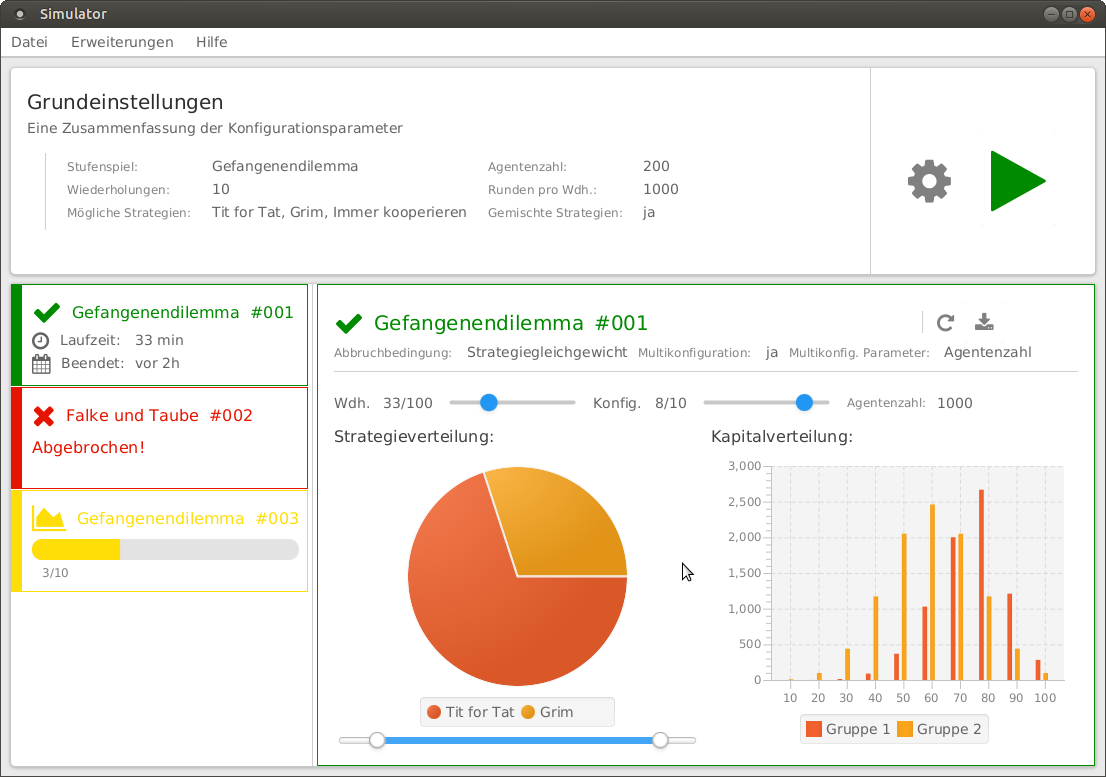
\includegraphics[width=\textwidth]{images/home.png}
	\caption{\label{fig:home}
		Hauptfenster des Simulators}
\end{figure}

Im oberen Drittel des Fensters wird eine Zusammenfassung der aktuell ausgewählten Konfiguration angezeigt (siehe \cref{fig:home_top}). Rechts davon befindet sich ein Knopf zum Bearbeiten der Konfiguration und ein weiterer Knopf zum Starten der Simulation (siehe \cref{fig:main_btn}).
 
\begin{figure}[hb]
	\centering
	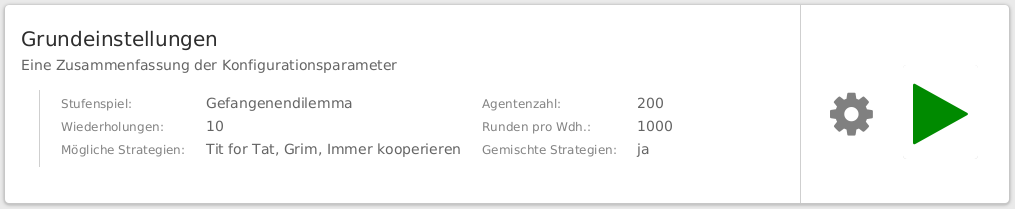
\includegraphics[width=\textwidth]{images/home_top.png}
	\caption{\label{fig:home_top}
	Zusammenfassung der aktuell gewählten Konfiguration}
\end{figure} 
 
\begin{figure}[ht]
	\centering
 	
\includegraphics[width=0.25\linewidth]{images/main_btn.png}
 	\caption{\label{fig:main_btn}
 		Knöpfe zum Konfigurieren und Starten einer Simulation}
\end{figure}


\newpage
Im unteren Teil des Fenster befindet sich links eine Historie der gelaufenen, abgebrochenen und noch laufenden Simulationen (siehe \cref{fig:history}). Wird ein Eintrag angeklickt, erscheint rechts eine Zusammenfassung der Ergebnisse der ausgewählten Simulation (siehe \cref{fig:home_output}). Mit den Knöpfen (siehe \cref{fig:out_btn}) kann die Simulation wiederholt werden und die detailierten Ergebnisse als \(.csv\) Datei exportiert werden. Mit Schiebereglern wird die Wiederholung und im Falle einer Multikonfiguration die Konfiguration ausgewählt, für welche die Ergebnisse angezeigt werden.



\begin{figure}[hb]
	\centering
	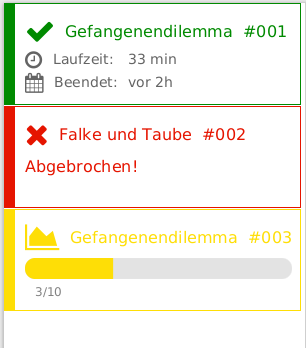
\includegraphics[height=0.5\linewidth ]{images/history.png}
	\caption{\label{fig:history}
		Simulationshistorie }
\end{figure}

\begin{figure}[ht]
	\centering
	
\includegraphics{images/out_btn.png}
	\caption{\label{fig:out_btn}
		Knöpfe zum Wiederholen und Exportieren der Ergebnisse einer Simulation}
\end{figure}
\begin{figure}[ht]
	\centering
	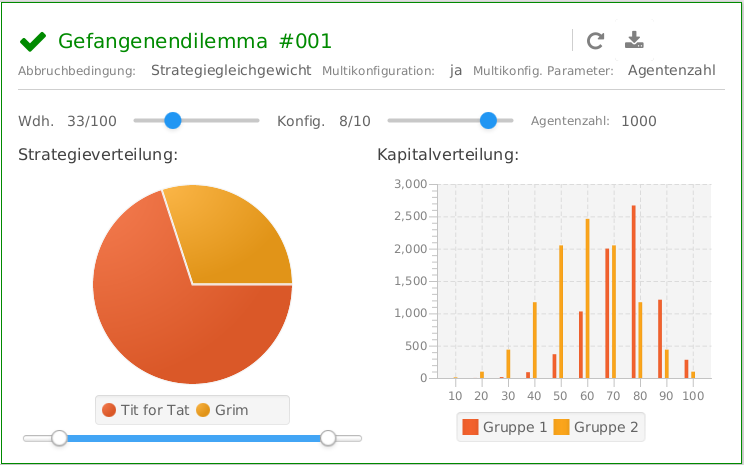
\includegraphics[width=\textwidth]{images/home_output.png}
	\caption{\label{fig:home_output}
		Ausgabe der Ergebnisse einer Simulation}
\end{figure}
\newpage
Über das Dateinmenü in der Menüleiste können Konfigurationen bearbeitet, gespeichert und geladen oder eine Simulation gestartet werden (siehe \cref{fig:menu1}).
Das Erweiterungsmenü enthält Optionen zum erstellen eines neuen Stufenspiels oder einer neuen Strategie (siehe \cref{fig:menu2}). Im Hilfemenü finden sich Bedienhilfen und Informationen über den Simulator (siehe \cref{fig:menu3}).

\begin{figure}[ht]
	\centering
	\subfloat[Dateimenü
	\label{fig:menu1}]{%
		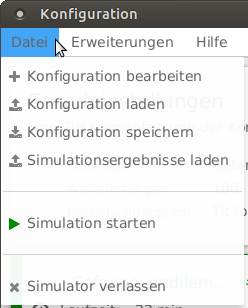
\includegraphics[height=0.25\linewidth]{images/Menu1.png}}
	\qquad
	\subfloat[Erweiterungsmenü
	\label{fig:menu2}]{%
		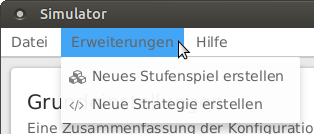
\includegraphics[width=0.25\linewidth]{images/Menu2.png}}
	\qquad
	\subfloat[Hilfemenü
	\label{fig:menu3}]{%
		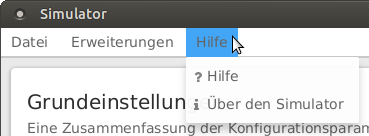
\includegraphics[width=0.25\linewidth]{images/Menu3.png}}
	\caption{\label{fig:menu}
		Funktionen der Menüleiste
	}
\end{figure}
\newpage
Drückt man den Knopf zum Bearbeiten einer Konfiguration, öffnet sich das Konfigurationsfenster (siehe \cref{fig:konfig}).

\begin{figure}[ht]
	\centering
	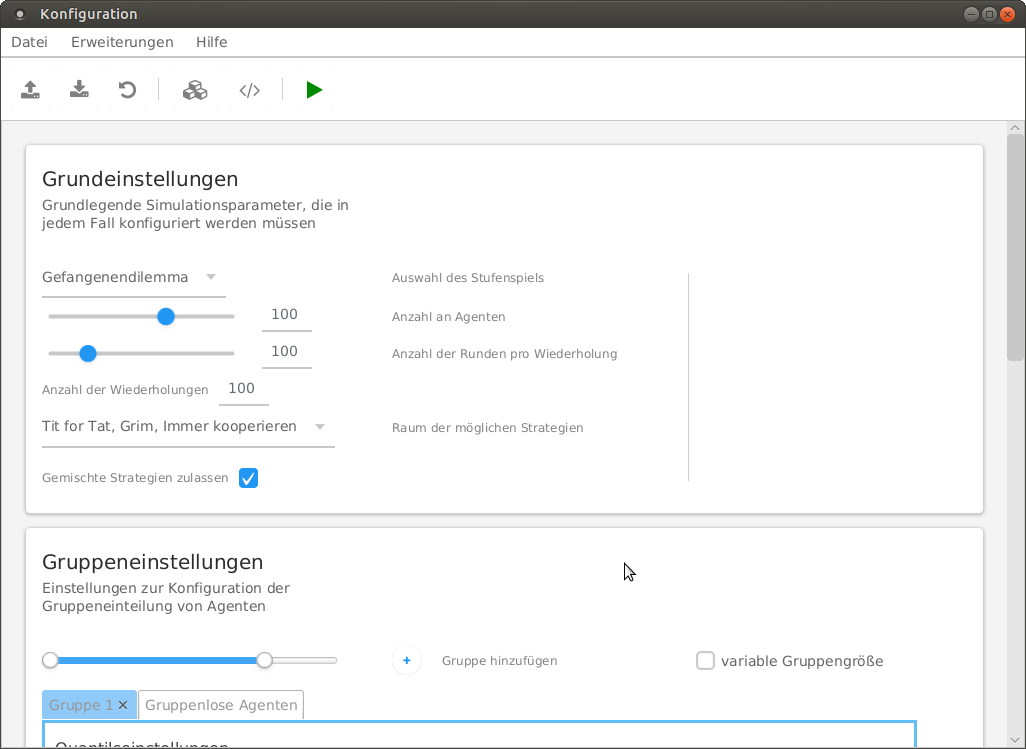
\includegraphics[width=\textwidth]{images/konfig.png}
	\caption{\label{fig:konfig}
		Konfigurationsfenster}
\end{figure} 

Das Konfigurationsfenster ist in drei Bereiche unterteilt, die jeweils ein- und ausgeklappt werden können:
\begin{itemize} \itemsep -10pt
	\item Grundeinstellungen
	\item Gruppeneinstellungen
	\item Erweiterte Einstellungen
\end{itemize}

Grundeinstellungen konfigurieren die fundamentalsten Simulationsparameter. Im rechten Teil wird das ausgewählte Stufenspiel in Normalform als Bimatrix dargestellt (siehe \cref{fig:konfig_main}). Über ein spezielles Dropdownmenü mit Checkboxen können für die Simulation zugelassene Strategien ausgewählt werden (siehe \cref{fig:konfig_strat_detail}).

\begin{figure}[ht]
	\centering
	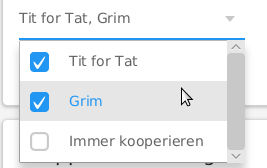
\includegraphics[width=0.25\textwidth]{images/konfig_strat_detail.png}
	\caption{\label{fig:konfig_strat_detail}
		Auswahl der zugelassenen Strategien}
\end{figure}

\begin{figure}[ht]
	\centering
	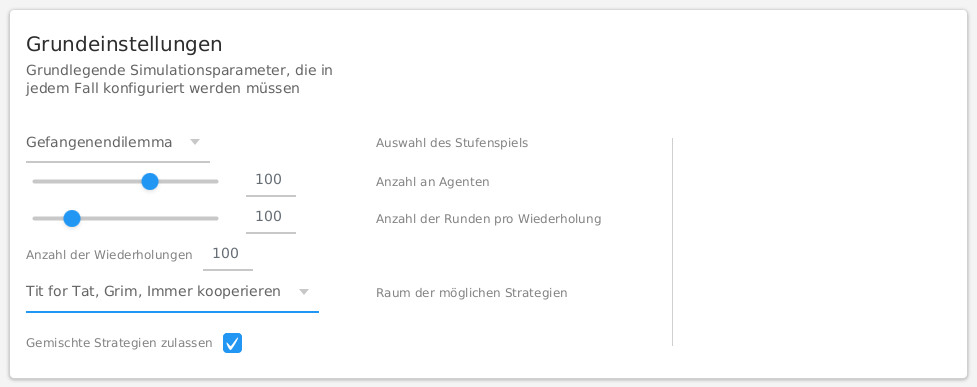
\includegraphics[width=\textwidth]{images/konfig_main.png}
	\caption{\label{fig:konfig_main}
		Grundeinstellungen im Konfigurationsfenster}
\end{figure}
\newpage
In den Gruppeneinstellungen können Gruppen angelegt und mit einem Multislider die Agenten frei in diese verteilt werden. Für jede Gruppe gibt es einen Tab (siehe \cref{fig:konfig_group}). Dort kann die Gruppe in gleicher Weise weiter in Segmente eingeteilt werden. Für jedes Segment kann das Startkapital der Agenten gemäß einer gewählten Verteilung festgelegt werden (siehe \cref{fig:konfig_cap} und die Initialstrategien eingestellt werden (siehe \cref{fig:konfig_strat}).



\begin{figure}[ht]
	\centering
	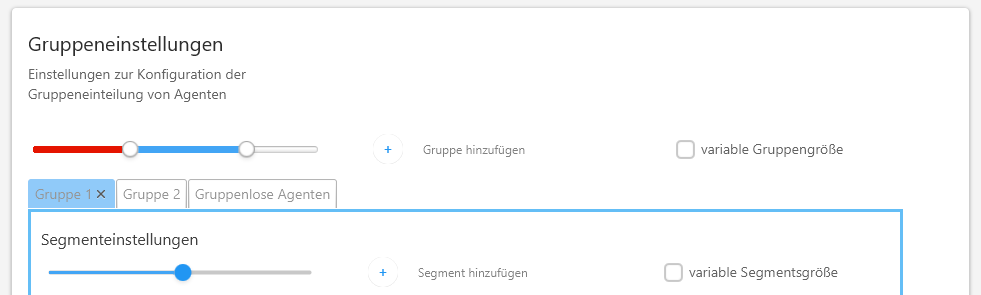
\includegraphics[width=\textwidth]{images/konfig_group.png}
	\caption{\label{fig:konfig_group}
		Gruppeneinstellungen im Konfigurationsfenster}
\end{figure}


In den erweiterten Einstellungen können spezialisierte Konfigurationen per Dropdowns eingestellt werden. Zudem kann hier der variable Konfigurationsparameter eingestellt werden, falls dieser in den Gruppen- bzw. Segementeinstellungen ausgewählt wurde. Dazu wird ein prozentualer Start- und Endwert angegeben und eine Schrittweite festgelegt \\(siehe \cref{fig:konfig_adv}). Hierdurch wird eine Multikonfiguration erstellt.

Am oberen Rand des Konfigurationsfenster befindet sich das gleiche Menü wie beim Hauptfenster (siehe \cref{fig:menu}) und darunter eine Werkzeugleiste (siehe \cref{fig:konfig_tool}). Über die Werkzeugleiste ist es möglich, Konfigurationen zu laden, zu speichern und die aktuelle Konfiguration auf die Standardwerte zurückzusetzen.\\Darüber hinaus gibt es hier Knöpfe zum Erstellen neuer Stufenspiele und Strategien. Eine Simulation mit der gewählten Konfiguration kann über die Werkzeugleiste gestartet oder das Konfigurationsfenster verlassen werden.

\begin{figure}[ht]
	\centering
	
\includegraphics[width=0.5\textwidth]{images/konfig_tool2.png}
	\caption{\label{fig:konfig_tool}
		Werkzeugleiste des Konfigurationsfenster}
\end{figure}

\begin{figure}[hb]
	\centering
	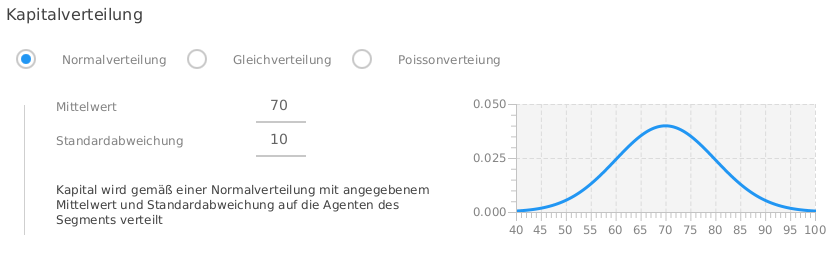
\includegraphics[width=\textwidth]{images/konfig_cap.png}
	\caption{\label{fig:konfig_cap}
		Auswahl der Kapitalverteilung für ein Segment}
\end{figure}

\begin{figure}[hb]
	\centering
	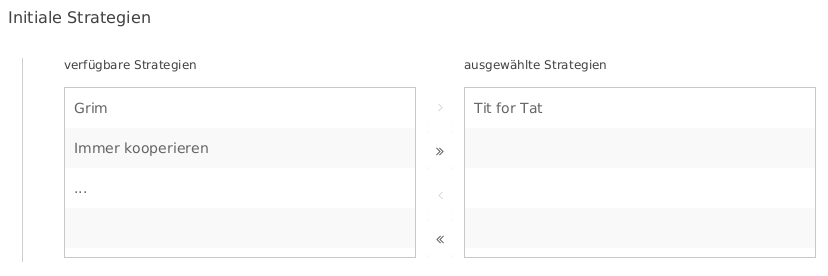
\includegraphics[width=\textwidth]{images/konfig_strat.png}
	\caption{\label{fig:konfig_strat}
		Auswahl der möglichen Initialstrategien für ein Segment}
\end{figure}

\begin{figure}[hb]
	\centering
	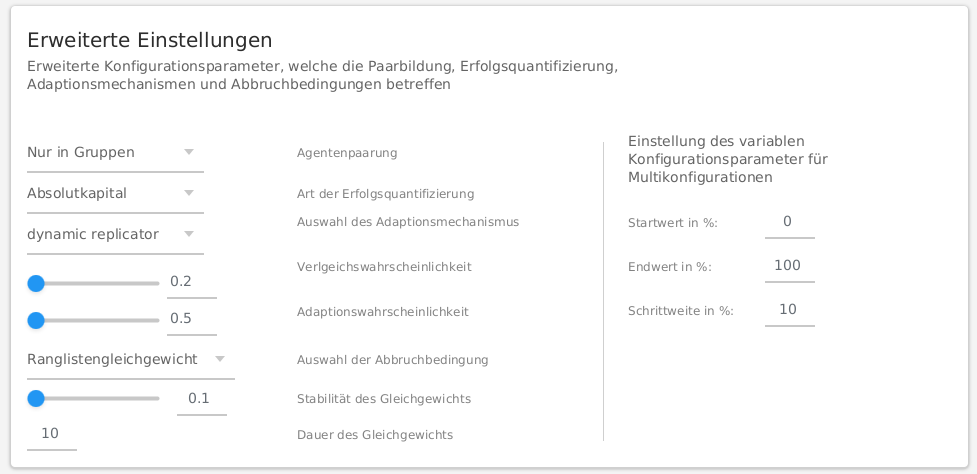
\includegraphics[width=\textwidth]{images/konfig_adv.png}
	\caption{\label{fig:konfig_adv}
		erweiterte Simulationsparameter und Multikonfigurationseinstellungen}
\end{figure}

\newpage

\section{Szenarien}

\subsection{Szenario 1}
Jonas hat die Anwendung auf seinem PC installiert und möchte das Stufenspiel Gefangenendilemma mit 10 Agenten simulieren, wobei von Anfang an eine Hälfte arm und eine Hälfte reich sein soll. Dazu öffnet Jonas die Anwendung und landet im Hauptfenster. Jonas drückt auf das Zahnrad um die von ihm gewünschte Konfiguration einzustellen. Das Konfigurationsfenster öffnet sich und Jonas wählt nun \enquote{Gefangenendilemma} bei der Auswahl des Stufenspiel aus und stellt den Slider bei Anzahl der Agenten auf 10. Die Anzahl der Runden und Wiederholungen lässt er auf den voreingestellten Werten. 
Um die Agenten jetzt in 2 Gruppen einzuteilen, erstellt Jonas unter Gruppeneinstellungen 2 neue Gruppen in dem er 2 mal auf das Plus mit \enquote{Gruppe hinzufügen} klickt. Er versetzt den Multislider nun so, dass in der einen Gruppe 6 Agenten sind und in der anderen Gruppe 4. Er klickt auf den Bereich des Multislider der an Gruppe 1 zugeteilt wurde und stellt im Unterpunkt Kapitalverteilung eine Normalverteilung mit Mittelwert 200 und Standardabweichung 5 ein. Gleiches tut er für Gruppe 2, jedoch wählt er hier als Mittelpunkt 40. Für beide Gruppen wählt er unter Strategieeinteilung nur \enquote{Grim}.
Jonas ist zufrieden mit seiner Konfiguration und startet diese nun mit einem Klick auf den grünen Play-Button in der Header-Leiste.
Er wird zurück ins Hauptfenster navigiert und sieht seine Simulation nun in der Simulationshistorie. Sie ist gelb eingefärbt (Sie läuft noch. Nach einer halben Stunde schaut Jonas noch mal nach, seine Simulation ist jetzt grün eingefärbt (Sie ist beendet). Mit einem Klick auf die Simulation öffnet Jonas die Zusammenfassung für seine Simulation und schaut sich nun die Kapitalverteilung für die einzelnen Gruppen an und wertet sie aus. Jonas ist zufrieden mit seinem Ergebnis und schließt die Anwendung wieder.


\subsection{Szenario 2}
Bob möchte eine Simulation des \enquote{Falke und Taube}-Stufenspiel mit 20 Agenten durchführen und die Verteilung der 2 Anfangsstrategien \enquote{Immer Kooperation} und Nie Kooperation so variieren lassen, dass in der ersten Simulation 10\% \enquote{Immer Kooperation} und 90\% \enquote{Nie Kooperation} als Anfangsstrategie haben und diese Verteilung sich in jeder Simulation um 10\% verschiebt(20:80, 30:70...). Dazu startet Bob die Anwendung und wählt das dementsprechende Stufenspiel und die Agentenzahl in den Grundeinstellungen. Den Raum der Strategien hat er auf \enquote{Nie Kooperation} und \enquote{Immer Kooperation} eingestellt und kann nun in den erweiterten Einstellungen seine Einstellung für den variablen Konfigurationsparameter treffen. Er stellt den Startwert auf 10\%, den Endwert auf 90\% und die Schrittweite auf 10\%. Er bestätigt die Konfiguration in dem er auf den grünen Haken in der Headerleiste klickt und gelangt zurück zum Hauptfenster. Im Hauptfenster kann er sich noch einmal die Zusammenfassung seiner aktuellen Konfiguration anschauen und überprüft ob er die wichtigen Dinge eingestellt hat. Nachdem er sich davon überzeugt hat, klickt er auf den grünen Play-Button um die Simulation zu starten. Er kann jetzt in der Simulationshistorie verfolgen wie viele von seinen 9 Simulationen schon beendet wurden. Nachdem alle Simulationen beendet sind, klickt er auf die Simulationsgruppe und kann sich nun eine Abstraktion der Simulationen anzeigen lassen um den Einfluss, den die Variation seines Parameter auf das Endergebnis hatte, auszuwerten. Bob findet ,dass diese eine interessante Auswirkung auf die Kapitalverteilung hatte und will die Konfiguration speichern um die Simulationen nächste Woche noch einmal durchzuführen. Dazu klickt er unter \enquote{Datei} auf \enquote{Konfiguration speichern} und kann nun einen Ablageort auswählen. Nach dem Speichern, schließt Bob die Anwendung und schickt die Konfigurationsdatei per E-Mail an seinen Kollegen Jonas, damit dieser die Simulation auch starten kann. Jonas kann die Konfiguration mittels \enquote{Konfiguration laden} öffnen und dann ganz normal starten.

\newpage
\section{Glossar}

\textbf{Gleichgewicht}:
Ein Gleichgewicht im Simulationsablauf ist erreicht, wenn keiner der Agenten mehr seine Strategie ändert.

\textbf{Stufenspiel:}
Ein spieltheoretisches Spiel, welches sich als Bimatrix darstellen lässt. (z.B. das Gefangenen-Dilemma)

\textbf{Bimatrix:}
Eine Matrix \(A \in (\mathbb{Z} \times \mathbb{Z})^{2 \times 2}\). Ein Stufenspiel wird eindeutig durch die Bimatrix seiner Auszahlungen definiert (siehe Anhang).

\textbf{Erfolg:}
Der Erfolg eines Agenten in einer Folge von Runden wird aus dessen Kapitalauszahlungen in diesen Runden berechnet. Er ist Konfigurationsparameter der Simulation. Beispiel ist die Summe aller Auszahlungen.

\textbf{Kapital:}
Jedem Agenten wird im Laufe einer Wiederholung eine Zahl zugeordnet, die sich aus dem Initialisierungswert zu Beginn der Wiederholung und der Summe der Auszahlungen aus den Stufenspielen der bisherigen Runden zusammensetzt.

\textbf{Gruppenzugehörigkeit:}
In einer Simulation sind die Agenten in eine feste, wohldefinierte Anzahl von Gruppen partitioniert. Die Strategien der Agenten können auf Gruppenzugehörigkeiten Bezug nehmen. Dabei haben zwei Agenten genau dann dieselbe Gruppenzugehörigkeit, wenn beide Mitglieder in derselben Gruppe sind. Insbesondere müssen beide Mitglied in einer Gruppe sein.

\textbf{Gruppenloser Agent:}
Ein Agent, der keiner Gruppe angehört.

\textbf{Konfiguration:}
Menge aller variablen Simulationsparameter. Diese sind in den Muss- und Kann-Kriterien aufgelistet.

\textbf{aktuelle Konfiguration:}
Die aktuelle Konfiguration ist die, mit der eine Simulation beim Betätigen des \enquote{Play}-Knopfes gestartet wird.

\textbf{Nutzer:}
Eine Person, welche das Programm nutzt.

\textbf{Multislider:}
Ein Schieberegler mit mehreren möglichen Schiebe-Knöpfen.

\textbf{Slider-Abschnitt:}
Bereich auf dem Slider, der nach rechts und links durch den nächstgelegensten Schiebe-Knopf bzw. den Rand des Sliders begrenzt wird.

\textbf{Strategie:}
Eine Strategie ist ein boole'scher Ausdruck (dessen Variablen von Spieler A und Gegenspieler B abhängen können), der bei Auswertung für zwei Spieler A und B genau dann wahr ist, wenn A unter Verwendung dieser Strategie beim Spiel gegen B kooperiert. Es folgt eine Liste aller Variablen, die in einer Strategie als Literal vorkommen können:
\begin{itemize}
\item A/B hat (bei bisherigen Spielen zwischen A und B im aktuellen \adapt) immer/nie/letztes Mal/wenigstens einmal kooperiert
\item B hat ein höheres/niedrigeres Absolutkapital als A
\item B hat einen höheren/niedrigeren Rang als A (im aktuellen \adapt)
\item A und B haben dieselbe Gruppenzugehörigkeit
\item A und B haben ähnliches Absolutkapital\footnote{Das Absolutkapital zweier Agenten ist ähnlich, genau dann wenn sich der Rang der Agenten, aufgelistet nach Absolutkapital, höchstens um \(20\%\) der Gesamtzahl aller Agenten unterscheidet.}
\item Die Konstanten true und false
Insbesondere sind Tit-for-Tat und Grim mögliche Strategien.
\end{itemize}

\textbf{Gemischte Strategie:}
Seien \(S_1,...,S_n\) die in einem Simulationsdurchlauf zugelassenen reinen Strategien. Eine gemischte Strategie ist dann ein Tupel \((\omega_1,...,\omega_n) \in \{0,\frac{1}{10},...,\frac{9}{10},1\}^n\) mit \(\sum_{i=1}^n \omega_i = 1\). \(\omega_i\) entspricht dann der Wahrscheinlichkeit, in einer Runde mit Strategie \(S_i\) zu spielen.

\textbf{Matching:}
Ein Matching der Menge \(\{1,...,N\}\) aller Agenten ist eine Menge \(M \subset \{\{i,j\} \subset \{1,...,N\} | i \neq j\}\), sodass gilt: \(\forall i \in \{1,...,N\}: \ |\{A \in M | i \in A\}| = 1\).

\end{document}
